\documentclass[conference]{IEEEtran}

\usepackage[T1]{fontenc}
\usepackage{lmodern}
\usepackage{microtype}
\usepackage{cite}
\usepackage{url}
\usepackage{xurl}
\usepackage[table]{xcolor}
\usepackage[hidelinks,hypertexnames=false]{hyperref}
\usepackage{booktabs}
\usepackage{tabularx}
\usepackage{array}
\usepackage{float}
\usepackage{graphicx}
\usepackage{amsmath}
\usepackage{amssymb}
\usepackage{listings}
\usepackage{caption}
\usepackage{tikz}
\usetikzlibrary{positioning,patterns,calc}

%% -------------------------------------------------------------------
%%  Allow slightly more flexible word-spacing in narrow columns so
%%  long multi-line section titles do not balloon inter-word gaps.
%%  We deliberately avoid \sloppy (it combines poorly with ragged
%%  columns and large tables; can trigger float-placement loops).
%% -------------------------------------------------------------------
\tolerance=1200
\emergencystretch=2.5em
\hbadness=10000

%% -------------------------------------------------------------------
%%  Professional color palette (muted, tier-1 journal appropriate)
%% -------------------------------------------------------------------
\definecolor{accent}{HTML}{1E3A8A}        % deep indigo, captions and rules
\definecolor{accentSoft}{HTML}{EEF2FF}    % pale indigo, table headers
\definecolor{codebg}{HTML}{F7F6F1}        % warm off-white, listing bg
\definecolor{codeframe}{HTML}{D5D2C8}     % warm grey, listing frame
\definecolor{codetitle}{HTML}{374151}     % slate, listing captions
\definecolor{kwcolor}{HTML}{7A4899}       % muted purple, keywords
\definecolor{typecolor}{HTML}{1D4E89}     % steel blue, types
\definecolor{strcolor}{HTML}{B45309}      % amber, strings
\definecolor{cmtcolor}{HTML}{6B7280}      % cool grey, comments
\definecolor{numcolor}{HTML}{0F766E}      % teal, numeric literals
\definecolor{sectioncolor}{HTML}{1D4E89}  % blue, TOML section headers

%% -------------------------------------------------------------------
%%  Typography and captions
%% -------------------------------------------------------------------
\renewcommand{\arraystretch}{1.06}
\captionsetup{font=small,labelfont={bf,color=accent},
              textfont=normalfont,skip=4pt}
\captionsetup[lstlisting]{font={small,color=codetitle},
              labelfont={bf,color=accent},
              textfont=normalfont,skip=3pt}
\setlength{\textfloatsep}{5pt plus 1pt minus 1pt}
\setlength{\floatsep}{4pt plus 1pt minus 1pt}
\setlength{\intextsep}{5pt plus 1pt minus 1pt}

%% -------------------------------------------------------------------
%%  Disable -- ligature in typewriter font so command flags like
%%  `--all` render as two hyphens rather than one en-dash.
%% -------------------------------------------------------------------
\DisableLigatures{encoding = T1, family = tt*}

%% -------------------------------------------------------------------
%%  Common table style: soft zebra striping, muted rules, ragged
%%  cells so narrow columns do not justify into awkward gaps. Every
%%  booktabs table invokes \tablesetup just after \begin{tabular}.
%% -------------------------------------------------------------------
\definecolor{tableHeaderBg}{HTML}{EEF2FF}  % pale indigo, header row
\definecolor{tableStripe}  {HTML}{F7F9FC}  % very pale blue-grey, even rows
\definecolor{tableRule}    {HTML}{B8BCC8}  % soft grey, horizontal rules

%% -------------------------------------------------------------------
%%  Envelope / opportunity chart palette.  Shared by fig:envelope and
%%  fig:warpos-opportunity so the two stacked charts read consistently.
%% -------------------------------------------------------------------
\definecolor{envBarGray}{HTML}{E5E7EB} % light gray, baseline / unrealized fill
\definecolor{envBar0}{HTML}{C2495E}    % muted rose-coral, per-agent task-core
\definecolor{envBar1}{HTML}{E89242}    % warm amber, Compress / +runtime
\definecolor{envBar2}{HTML}{4AA89A}    % teal, Suppress / +repository-native
\definecolor{envBar3}{HTML}{2A6F4D}    % deep jade, projected / +theoretical

% p{<width>}: left-aligned, ragged-right, top-aligned text cell
\newcolumntype{L}[1]{>{\raggedright\arraybackslash}p{#1}}

% Invoke at the top of every tabular for consistent row spacing and
% softer horizontal rules. We deliberately do NOT call \rowcolors here
% because it interacts badly with table*[t] floats that span both
% columns, sometimes provoking a float-placement loop.
\newcommand{\tablesetup}{%
  \renewcommand{\arraystretch}{1.15}%
  \arrayrulecolor{tableRule}%
}

\newcommand{\tighttablesetup}{%
  \renewcommand{\arraystretch}{1.06}%
  \setlength{\tabcolsep}{4pt}%
  \arrayrulecolor{tableRule}%
}

\newcommand{\concepttag}[1]{%
  \noindent{\small\ttfamily #1}\par\vspace{2pt}%
}

%% -------------------------------------------------------------------
%%  Syntax-highlighted listing languages and styles
%% -------------------------------------------------------------------
\lstdefinelanguage{RustLang}{
  morekeywords={fn,let,pub,mut,impl,struct,enum,trait,match,if,else,
    for,while,loop,return,use,mod,const,static,type,crate,self,Self,
    super,async,await,move,ref,as,where,dyn,extern,unsafe,true,false,
    break,continue,in,box},
  morekeywords=[2]{i8,i16,i32,i64,u8,u16,u32,u64,usize,isize,bool,
    char,f32,f64,str,String,Result,Option,Vec,Box,Rc,Arc,HashMap,
    BTreeMap,Mutex,RwLock,Send,Sync,Iterator,Error,Display,Debug,
    Clone,Copy,Default,UserId,LoadUserError,Job,Timestamp,JobError,
    Task,TaskState,DomainError,User},
  sensitive=true,
  morecomment=[l]{//},
  morecomment=[s]{/*}{*/},
  morestring=[b]"
}

\lstdefinelanguage{TomlLang}{
  morecomment=[l]{\#},
  morestring=[b]",
  sensitive=true
}

\lstdefinelanguage{TreeLang}{
  morecomment=[l]{\#},
  sensitive=true
}

\lstdefinestyle{basebox}{
  basicstyle=\ttfamily\footnotesize,
  breaklines=true,
  breakatwhitespace=false,
  columns=fullflexible,
  keepspaces=true,
  showstringspaces=false,
  backgroundcolor=\color{codebg},
  frame=single,
  framerule=0.5pt,
  rulecolor=\color{codeframe},
  framesep=4pt,
  xleftmargin=4pt,
  xrightmargin=4pt,
  aboveskip=5pt,
  belowskip=5pt,
  captionpos=b,
  numbers=none,
  abovecaptionskip=2pt,
  belowcaptionskip=6pt
}

\lstdefinestyle{rustcode}{
  style=basebox,
  language=RustLang,
  keywordstyle=\color{kwcolor}\bfseries,
  keywordstyle=[2]\color{typecolor},
  commentstyle=\color{cmtcolor}\itshape,
  stringstyle=\color{strcolor}
}

\lstdefinestyle{tomlcode}{
  style=basebox,
  language=TomlLang,
  keywordstyle=\color{sectioncolor}\bfseries,
  commentstyle=\color{cmtcolor}\itshape,
  stringstyle=\color{strcolor},
  moredelim=**[is][\color{sectioncolor}\bfseries]{[}{]}
}

\lstdefinestyle{treecode}{
  style=basebox,
  language=TreeLang,
  commentstyle=\color{cmtcolor}\itshape
}

\lstdefinestyle{plaincode}{
  style=basebox,
  commentstyle=\color{cmtcolor}\itshape,
  keywordstyle=\color{typecolor}\bfseries,
  stringstyle=\color{strcolor}
}

%% -------------------------------------------------------------------
%%  Paper-specific macros (wrap in \textnormal so small caps survive
%%  italic or bold contexts without triggering font-shape warnings)
%% -------------------------------------------------------------------
\newcommand{\ari}{\textnormal{\textsc{ARI}}}
\newcommand{\etts}{\textnormal{\textsc{ETTS}}}
\newcommand{\secureetts}{\textnormal{\textsc{SecureETTS}}}
\newcommand{\mss}{\textnormal{\textsc{MSS}}}

\title{Minimum Semantic Surface:\\A Token-Aware Operating Standard for Agent-Efficient Rust Codebases}

\author{
\IEEEauthorblockN{Jepson Taylor}
\IEEEauthorblockA{
\textit{Research Group}\\
\textit{VEOX Inc.}\\
jepson@veox.ai
}
}

\begin{document}

%% -------------------------------------------------------------------
%%  Title, decorative rules, full-width abstract, hero figure.
%%  All spanning both columns via \twocolumn[...] + @twocolumnfalse;
%%  two-column body resumes after.  Inside @twocolumnfalse we avoid
%%  \begin{center} (which disturbs paragraph mode) and prefer minipage
%%  + \centering.
%% -------------------------------------------------------------------
\makeatletter
\twocolumn[{%
\begin{@twocolumnfalse}%

\maketitle

% Single decorative rule below the title (thin accent)
\vspace{-2pt}
\noindent\textcolor{accent}{\rule{\linewidth}{0.7pt}}\par
\vspace{4pt}

\begin{abstract}
\noindent Repository-scale coding agents fail less from syntax ignorance than from repository-control errors: wrong owner, hidden contract, wrong proof lane, setup friction, noisy evidence, retry burn, and security-blind success. We propose \emph{minimum semantic surface} (\mss) as a review-backed Rust operating standard: expose the smallest high-signal set of navigation, contract, proof, diagnostic, and policy artifacts needed for a valid change. Rust is a strong substrate because ownership, typed APIs, module privacy, Cargo metadata, compiler diagnostics, and supply-chain tooling convert architectural boundaries into executable constraints rather than ambient prose. The paper synthesizes repository-agent, Rust-specific, context, security, and tooling evidence; defines \mss{} and its canonical artifacts; and specifies token discipline, proof lanes, and review receipts for repositories that aim to export the smallest lawful repair program while preserving correctness, security-gated validation, auditability, and human review. A bounded runtime mediation layer is discussed only as companion evidence for residual waste classes that can still survive after repository shape has been disciplined; it is not presented as core proof of \mss{}.
\end{abstract}

\begin{IEEEkeywords}
\noindent Rust, coding agents, token efficiency, software architecture, repository-scale repair, verification, software security, developer productivity
\end{IEEEkeywords}

\vspace{5pt}

%% -------------------------------------------------------------------
%%  Hero figure: lawful repair path.  Wrapped in a minipage with
%%  \centering (safer than \begin{center} inside @twocolumnfalse).
%% -------------------------------------------------------------------
\noindent\begin{minipage}{\linewidth}
\centering
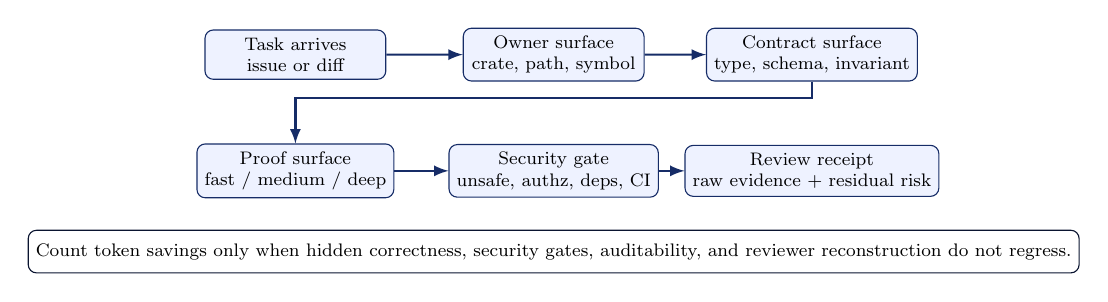
\begin{tikzpicture}[
    scale=0.82, transform shape,
    stage/.style = {
      draw=accent!75!black,
      fill=accentSoft,
      rounded corners=3pt,
      minimum width=2.8cm,
      minimum height=0.72cm,
      align=center,
      font=\footnotesize
    },
    note/.style = {
      draw=accent!35!black,
      fill=white,
      rounded corners=3pt,
      minimum width=5.8cm,
      minimum height=0.66cm,
      align=center,
      font=\footnotesize
    },
    arrow/.style = {-latex, thick, draw=accent!75!black}
  ]
\node[stage] (task) at (0, 1.25) {Task arrives\\issue or diff};
\node[stage] (owner) at (4.0, 1.25) {Owner surface\\crate, path, symbol};
\node[stage] (contract) at (8.0, 1.25) {Contract surface\\type, schema, invariant};

\node[stage] (proof) at (0, -0.55) {Proof surface\\fast / medium / deep};
\node[stage] (security) at (4.0, -0.55) {Security gate\\unsafe, authz, deps, CI};
\node[stage] (receipt) at (8.0, -0.55) {Review receipt\\raw evidence + residual risk};

\draw[arrow] (task) -- (owner);
\draw[arrow] (owner) -- (contract);
\draw[arrow] (contract.south) -- ++(0,-0.25) -| (proof.north);
\draw[arrow] (proof) -- (security);
\draw[arrow] (security) -- (receipt);

\node[note] (safe) at (4.0, -1.8) {Count token savings only when hidden correctness, security gates, auditability, and reviewer reconstruction do not regress.};
\end{tikzpicture}

\vspace{3pt}
\captionof{figure}{Failure funnel and lawful repair path under \mss{}. The repository should answer owner, contract, proof, and evidence-preservation questions before broad edits or broad validation.}
\label{fig:hero}
\end{minipage}

\vspace{6pt}
\vfill
\pagebreak

\end{@twocolumnfalse}%
}]
\makeatother

% Backup forced page break so the two-column body (Introduction onward)
% begins on page 2. The \vfill+\pagebreak inside the \twocolumn[...]
% preamble ends the single-column region with a page boundary; the
% \clearpage here guarantees it even if the preamble break is absorbed.
\clearpage

\section{Introduction}
Coding agents rarely fail because they cannot emit Rust syntax. They fail because the repository does not tell them, early and cheaply, \emph{who} owns a surface, \emph{what} contract must remain true, \emph{how} a change is proved, and \emph{what} evidence must not be hidden. A typical failure trace is now familiar: broad search, wrong file, plausible patch, visible green, hidden invariant miss, then a second round spent reconstructing what should have been explicit at the outset.

Repository-scale agent work is therefore a repository-interface problem as much as a model problem. SWE-bench established execution-based issue repair, and SWE-agent showed that navigation, editing, and testing interfaces materially change outcomes \cite{sweBench2024,sweAgent2024}. Subsequent work broadens the question from ``can a model patch?'' to ``can a system reach correct, security-gated, reviewable change at acceptable cost?'' \cite{sweEffi2025,susvibes2025}. Context studies sharpen the same point: more retrieved text is not automatically better, because agents over-retrieve, under-use explored context, and can be harmed by broad instruction files or mismatched skill packs \cite{contextBench2026,agentsMdEval2026}. Careful workflow studies are equally sobering: experienced open-source developers were measured slower on their own repositories with early-2025 AI tooling, and more recent field work finds that professional developers supervise, scope, and control agent loops rather than let them run free \cite{metrProductivity2025,professionalControl2025}.

Rust deserves focused treatment because, in agentic development, the programming language is part of the control system. Ownership, enums, traits, module privacy, Cargo workspaces, compiler diagnostics, tests, and typed errors can make architectural boundaries executable rather than merely described. Rust-SWE-bench and RUSTFORGER quantify the Rust-specific bottleneck directly: across 500 issue-resolution tasks drawn from 34 real Rust repositories, the RUSTFORGER baseline resolves 21.2\% of tasks and the reported configuration reaches 28.6\%, with repository structure, strict type/trait semantics, and issue reproduction named as the dominant remaining obstacles \cite{rustSweBench2026}. RustEvo2 and RustAssistant expose adjacent difficulty and opportunity in API evolution and compiler-guided repair \cite{rustEvo2025,rustAssistant2025}. Production reports further show that Rust is already used where the cost of wrong changes is high: Google's 2025 Android Rust post reports roughly \textbf{1000$\times$} lower memory-safety vulnerability density, \textbf{$\sim$4$\times$} lower rollback rate, and \textbf{$\sim$25\%} less code-review time versus Android C/C++ changes \cite{googleAndroid2025}, and Cloudflare, AWS, Firecracker, and Hugging Face Tokenizers corroborate the substrate maturity story \cite{cloudflareRust2025,awsRust2022,firecracker2026,hfTokenizers2026}. These production cases do not prove agent efficiency directly; they prove that Rust is mature enough that repository-control improvements matter.

This paper takes a bounded stance. Rust is not always easiest for agents to write and not always cheapest by raw token count. It is a strong mainstream default when mistake cost dominates first-edit speed: security-sensitive services, parsers, protocol code, CLIs, infrastructure tools, long-lived libraries, and concurrency-heavy systems.

The paper's contribution is a review-backed operating standard for such codebases. It defines the vocabulary and review discipline needed to separate evidence, project claims, and doctrine, and it maps common agent failure stages to concrete Rust repository controls. It specifies canonical repository artifacts, proof lanes, token-accounting rules, and reviewer receipts. A bounded runtime companion layer appears later only to show which residual waste classes remain visible once repository shape has already been disciplined. It closes with three buildable future systems (\texttt{cargo-mss}, \texttt{ProofLens}, and \texttt{cargo-obligation-cache}) that could materially shrink navigation waste, proof-output waste, and repeated-proof waste without weakening correctness or security.

\section{Review Method and Evidence Taxonomy}
\label{sec:method}
This manuscript is a review and operating standard, not a local benchmark report. Because no counts of screened or excluded sources are reported, the protocol below is labeled a \emph{structured review protocol} rather than a full PRISMA-style systematic review. Its role is to make evidence classes explicit so the reader can audit which later claims are public, official, project-reported, or doctrinal.

\noindent\textbf{Source classes searched (7).} (i)~repository-agent benchmarks and failure analyses; (ii)~Rust-specific repair and migration studies; (iii)~context, pruning, and token-efficiency work; (iv)~harness and tool-interface guidance from major agent platforms; (v)~official Rust and Cargo documentation; (vi)~first-party production Rust engineering posts; (vii)~project documentation for tools that directly affect proof cost, contract drift, or token shaping.

\noindent\textbf{Search themes.} Repository repair, Rust-specific repair, context pruning, repository-level instruction files, continuous integration, build-loop acceleration, supply chain, secure agent operation.

\noindent\textbf{Date window.} Primary search closed April 23, 2026; live refresh windows are tracked per-claim in the supplement claim ledger.

\noindent\textbf{Inclusion rules.} (a)~primary peer-reviewed studies and preprints with described method; (b)~official project and standards-body documentation; (c)~first-party engineering posts when used as production-substrate evidence; (d)~tool documentation when used as mechanism-plausibility evidence.

\noindent\textbf{Exclusion rules.} (a)~anonymous summaries; (b)~vendor leaderboard claims without method; (c)~listicle-style roundups; (d)~crate recommendations justified only by popularity.

\noindent\textbf{Evidence classes.} Six, labeled explicitly in-text: \emph{direct} evidence (Rust-agent or repo-agent studies), \emph{adjacent} evidence (context, security, workflow, cost), \emph{mechanism} evidence (official Rust/Cargo and tool docs), \emph{production substrate} evidence (first-party engineering posts), \emph{project claim} evidence (tool or repo docs as plausible mechanism, not proof), and \emph{proposed doctrine} (this paper's synthesis).

\noindent\textbf{Risk-of-bias sentence.} Company engineering posts select for publishable wins, project documentation selects for mechanism favorability, and popular benchmarks carry contamination risk as they leak into training data; we call these out in-line where they materially affect a claim.

These rules drive two editorial conventions applied throughout the paper. First, token-reduction claims from project materials are treated as project-reported unless they have been validated under hidden- and security-gated criteria \cite{rtk2026}. Second, repository-level instruction files are cited as routing mechanisms, not as free wins: evaluation work shows that broad or mismatched instruction content can \emph{reduce} task success and increase inference cost, so the standard favors short, local, and executable guidance \cite{agentsMdEval2026,openaiAgents2026,githubCopilotInstructions2026}. Later sections follow one simple evidence split: public and official sources justify the standard itself, while WarpOS-style runtime evidence is bounded to local corpus observations about residual waste and buildable intervention surfaces. Proposed review triggers, code-shape budgets, and token policies are labeled doctrine rather than external fact.

\section{Agent Failure Funnel}
\label{sec:failure}
Minimum semantic surface starts from a failure model. Agents do not merely ``need context''; they fail at identifiable stages, each of which has a corresponding repository control and a measurable metric. Table~\ref{tab:failure-funnel} is the load-bearing artifact for the rest of the paper: every later prescription maps back to exactly one row. Failures often progress through six stages --- \emph{wrong owner}, \emph{wrong contract}, \emph{wrong patch scope}, \emph{wrong proof lane}, \emph{unsafe evidence compression}, \emph{security-blind success}, and a \emph{reviewer-reconstruction tax} that charges the human even when the patch is nominally correct --- though a given session can enter at any stage. Each stage is an independent failure class: fixing owner discovery does not close the security gate, and compressing tool output does not fix wrong-owner edits.

\begin{table*}[t]
  \centering
\caption{Agent failure funnel, motivating evidence, and Rust repository response}
\label{tab:failure-funnel}
  \resizebox{\textwidth}{!}{
  \tablesetup
  \begin{tabular}{>{\raggedright\arraybackslash}p{0.15\textwidth}>{\raggedright\arraybackslash}p{0.28\textwidth}>{\raggedright\arraybackslash}p{0.27\textwidth}>{\raggedright\arraybackslash}p{0.22\textwidth}}
    \toprule
    \rowcolor{tableHeaderBg}
    failure stage & typical agent symptom & motivating evidence & Rust repository response \\
    \midrule
    wrong owner & broad search, wrong crate, many files opened & localization and graph-guidance work \cite{agentless2024,locAgent2025,repoGraph2024} & owner map, narrow crates, test map, rust-analyzer navigation \\
    \rowcolor{tableStripe}
    hidden contract & visible pass, hidden invariant regression & Rust repair and migration work \cite{rustSweBench2026,rustEvo2025,rustAssistant2025} & newtypes, private fields, validated constructors, generated contracts, local tests \\
    wrong patch scope & broad speculative patch; cross-crate drift & AGENTS.md and context studies \cite{contextBench2026,agentsMdEval2026,anthropicContext2025} & legal edit zones, generated-zone markers, widening rules \\
    \rowcolor{tableStripe}
    wrong proof lane & too little validation or whole-workspace thrash & setup, CI, and harness studies \cite{setupBench2025,sweCi2026,openaiHarness2026} & canonical proof lanes, change-type routing, one-command setup \\
    noisy evidence & compiler/test/log output dominates context & cost and pruning work \cite{sweEffi2025,swePruner2026,anthropicTools2025} & JSON diagnostics, failure-first summaries, raw-output tee \\
    \rowcolor{tableStripe}
    security-blind success & functional patch remains exploitable & secure-correctness and standards \cite{susvibes2025,owaspLlmTop102026,owaspAgentSecurity2026,nistSsdf2022,openssfScorecard2026} & security-gated lanes, secret scanning, unsafe ledger, dependency review \\
    reviewer reconstruction tax & human cannot reproduce why a change is correct & workflow and productivity research \cite{metrProductivity2025,professionalControl2025,spaceFramework2021} & proof receipts, contract diffs, stable diagnostic codes \\
    \bottomrule
  \end{tabular}}
\end{table*}

Three observations follow. First, the funnel is \emph{ordered}: a patch cannot be correct until the owner is right, cannot be hidden-passing until the contract is right, and cannot be ship-safe until the security lane passes. Second, each row maps to at least one repository artifact the standard will prescribe later, so the failure model is what the rest of the paper satisfies, not narrates. Third, the same row indexes both the evidence synthesis in the next section and the validation ladder in \S\ref{sec:proof}, so reviewers can traverse the paper by failure stage rather than by section number.

\noindent\textbf{Worked trace: one issue through all six stages.} Consider a small-but-realistic billing issue: \emph{``grace-period users are billed one cycle early when they upgrade plans.''} An unprepared agent begins with a repository-wide search for ``grace'' (\textbf{wrong owner}: 40+ files opened, most in the web layer) and proposes a patch in \texttt{api-server/routes/billing.rs} that changes a status-code mapping (\textbf{wrong contract}: the invariant lives in \texttt{crates/billing-domain/src/plan\_change.rs}, gated by a private constructor). Workspace tests pass (\textbf{unsafe evidence compression}: the domain unit test that exercises the boundary is not triggered because the patch is upstream of it) and a full \texttt{cargo test --workspace} is run to ``be sure'' (\textbf{wrong proof lane}: 9~min vs the 70~s fast lane scoped to \texttt{-p billing-domain}). Review catches the functional bug, but the dependency upgrade that shipped with it introduces a known advisory (\textbf{security-blind success}); the reviewer then spends another 30~min reconstructing which commands were run and against which commit (\textbf{reviewer reconstruction tax}). An \mss{}-compliant repository turns every one of those stages into a local artifact lookup: the owner map names \texttt{billing-domain} as owner of grace-window logic; the generated contract names the one function whose signature must remain stable; \texttt{just fast -p billing-domain} is the canonical fast lane; the security lane surfaces the advisory on the same CI gate; and the proof receipt emits the commands, hashes, and owners so the reviewer reads one page instead of replaying one hour.

\section{Evidence Landscape}
\label{sec:evidence}
Three evidence families do the most work for the token-aware standard. ContextBench reports that explored and actually used context diverge materially on repository tasks, which argues for routing and pruning rather than indiscriminate long context \cite{contextBench2026}. SWE-Effi argues that time and token cost belong in evaluation rather than as afterthoughts, which grounds the paper's \etts{} and \secureetts{} objectives \cite{sweEffi2025}. SUSVIBES shows that functional success and secure success diverge badly on real-world tasks, which is why security must be a separately gated proof lane \cite{susvibes2025}.

Rust-specific work tightens the picture. Rust-SWE-bench and RUSTFORGER identify repository structure, strict type and trait semantics, and issue reproduction as first-order difficulties \cite{rustSweBench2026}. RustAssistant, AutoVerus, and Debug2Fix show that compiler diagnostics and proof generation are usable levers for narrowing agent edits, not merely decorative \cite{rustAssistant2025,autoVerus2024,debug2Fix2026}. RustEvo2 emphasizes that API evolution and safe migration are recurring confusion surfaces \cite{rustEvo2025}. Recent scaffolding work shows that repository layout itself shapes LLM agent behavior before any prompt is read \cite{insideScaffold2026}. Harness guidance from OpenAI and Anthropic converges on three mechanical levers: short and executable agent-facing instructions, context preservation across long runs, and tool interfaces that summarize without hiding evidence \cite{openaiHarness2026,openaiAgents2026,anthropicTools2025}.

The convergent lesson is that agents fail less from lack of code-generation capacity than from poor repository interfaces: poor owner discovery, poor proof routing, poor setup, and poor evidence shaping. Repository-agent benchmarks motivate owner maps, one-command setup, and proof-lane routing; Rust-specific studies motivate typed contracts and generated boundaries; context work motivates short routers and bounded manifests; harness guidance motivates machine-readable diagnostics and raw-evidence paths; and security plus workflow work motivates a separate security gate and reviewer receipts \cite{sweAgent2024,rustSweBench2026,contextBench2026,openaiHarness2026,susvibes2025,professionalControl2025}. That lesson is the scaffolding for the \mss{} standard.

\section{Why Rust, and When Not Rust}
\label{sec:why-rust}
Rust is not the easiest language for agents to write. It is one of the best languages for making wrong agent edits fail early, locally, and diagnostically. Ownership and borrowing express aliasing constraints; enums express closed state; traits expose capability surfaces; module privacy limits accidental reach; Cargo exposes a machine-readable workspace graph; and the ecosystem provides well-documented tools for features, APIs, unsafe code, contracts, tests, and supply chain \cite{rustApiGuidelines2026,cargoWorkspaces2026,cargoMetadata2026}.

Production evidence shows substrate maturity rather than agent efficiency: Android reports lower rollback and memory-safety burden after migration, Cloudflare reports operational wins in hot paths, Firecracker shows Rust in invariant-heavy systems, AWS uses it in infrastructure, and Hugging Face uses it in AI-adjacent performance-critical tooling \cite{googleAndroid2025,googleAndroid2022,cloudflareRust2025,firecracker2026,awsRust2022,hfTokenizers2026}. The language-choice rule is comparative. Rust should own invariant-heavy, security-sensitive, concurrency-sensitive, and latency-sensitive cores. It is not the right tool everywhere: TypeScript remains the practical default for mainstream UI surfaces, Python for exploratory data and ML glue, Go for straightforward operational services, JVM/.NET ecosystems for large enterprise integration surfaces, and C/C++ or Zig for hardware or legacy edges.

\noindent\textbf{Default pairing.} Rust is not always the lowest-token language; it is the best default when the expected cost of mistakes exceeds the cost of stricter contracts. For typical product systems the paper's explicit recommendation is \emph{Rust backend + TypeScript/React frontend + generated contracts at the boundary} (OpenAPI or Protobuf, with runtime validation on the JS side); Tauri for desktop shells, Python via PyO3 or maturin for exploratory or packaging edges, tonic/prost or Buf for service contracts, and wasm-pack for browser-side deployment round out the surface. Polyglot is not the enemy; untyped polyglot boundaries are.

\section{Minimum Semantic Surface Standard}
\label{sec:mss}
\mss{} is the smallest high-signal repository structure that answers \emph{owner, contract, proof, diagnostic,} and \emph{policy} questions before an agent edits broadly. The goal is not minimum text; it is minimum ambiguity at the point of change.

\subsection{The Five Surfaces}
We decompose \mss{} into five surfaces. The \emph{navigation surface} answers where to look. The \emph{contract surface} answers what must remain true. The \emph{proof surface} answers how to falsify a current theory. The \emph{diagnostic surface} answers what a failure means. The \emph{policy surface} answers what must not be edited, skipped, or hidden. A \emph{lawful repair program} is the smallest traversal of these surfaces that suffices for a valid change.

The standard is deliberately strict. Navigation \textbf{must} name owners and keep one reason to change per crate or module; contract surfaces \textbf{must} generate or test public schemas and mark generated zones; proof surfaces \textbf{must} publish fast, medium, deep, and security lanes as commandable tasks; diagnostic surfaces \textbf{must} preserve exit codes, primary spans, and failing-test identity; and policy surfaces \textbf{must} keep root instructions short while requiring rationale for dependency, unsafe, or CI changes. The corresponding \textbf{must not} rules are equally important: do not hide ownership in \texttt{utils} or \texttt{helpers}, do not hand-edit generated output without updating its source of truth, do not accept green-looking summaries without raw evidence, and do not force the agent to reconstruct repository policy from CI YAML.

\subsection{Canonical Repository Shape}
The canonical \mss{} repository keeps invariants in narrow domain crates, pushes I/O to adapters, separates generated from handwritten code, and publishes agent-facing artifacts under a machine-readable \texttt{agent/} directory. The root \texttt{AGENTS.md} routes rather than teaches: it points the agent to owners, canonical commands, forbidden zones, and raw-evidence policy without becoming a second manual \cite{agentsMdEval2026,onImpactAgents2026,openaiAgents2026,anthropicMemory2026}. Listings~\ref{lst:tree} and~\ref{lst:agents} show a minimal viable shape; the supplement carries an extended tree, a fuller \texttt{AGENTS.md} example, and an illustrative \texttt{proof-lanes.toml}.

\begin{lstlisting}[style=treecode,caption={Canonical \mss{} workspace tree (compact)},label={lst:tree}]
repo/
  AGENTS.md  Cargo.toml  rust-toolchain.toml  justfile
  proof-lanes.toml
  agent/
    agent-map.json  test-map.json  contract-map.json
    unsafe-ledger.toml  generated-zones.toml
  crates/{domain,application,adapters,api,cli}/
  contracts/  generated/  tests/  fuzz/  benches/
  artifacts/raw/
\end{lstlisting}

\begin{lstlisting}[style=plaincode,caption={Canonical root \texttt{AGENTS.md} (excerpt)},label={lst:agents}]
Mission: invariants live in crates/domain.
Start: just fast.  Handoff: just medium.
Map: domain=logic; application=use cases; adapters=I/O.
Forbidden: generated/ and paths in agent/generated-zones.
Never compress: exit code, failing test name,
panic text, span, advisory ID, fuzz seed,
raw-log path, raw-log hash.
Security lane: authz, secrets, unsafe, FFI, CI/CD, shell.
\end{lstlisting}

The governing rules are what matters: generated zones must be explicit, root instructions must stay short, proof lanes must be commandable rather than prose, and raw output must remain recoverable by stable path or hash.

\section{Agent-Efficient Rust Architecture}
\label{sec:design}
The design rules that keep agents on the rails convert architecture into executable constraints. Most are standard Rust practice; we state them explicitly because an agent will not infer them from prose.

\subsection{Four Canonical Micro-Patterns}
The recurring patterns are small and conservative. Each narrows the legal edit zone and concentrates the first failing proof on one owner, so an agent that misreads the surface is corrected by \texttt{rustc} rather than by a reviewer. The canonical four are typed IDs instead of naked strings, validated constructors instead of public mutable structs, enums instead of boolean state bundles, and typed errors with stable codes instead of stringly failure channels. The small excerpts below show each pattern as a before/after contrast; the supplement carries fuller examples.

\noindent\textbf{Typed IDs.} Raw strings lose their identity at the function boundary and invite silent mix-ups between users, orders, and sessions. A newtype keeps the compiler honest and gives the agent a single place to land a validation fix.

\begin{lstlisting}[style=rustcode,caption={Typed ID: before and after},label={lst:typed-id}]
// before: any string passes typecheck
fn load_user(id: String) -> User { /*...*/ }

// after: only UserId satisfies the signature
#[derive(Debug, Clone, PartialEq, Eq, Hash)]
pub struct UserId(String);
impl UserId {
    pub fn parse(s: &str) -> Result<Self, DomainError> {
        if s.starts_with("u_") && s.len() <= 36 {
            Ok(Self(s.to_owned()))
        } else { Err(DomainError::BadUserId) }
    }
}
fn load_user(id: UserId) -> User { /*...*/ }
\end{lstlisting}

\noindent\textbf{Validated constructor.} Public mutable fields let a patch skip the invariant even when the invariant is documented. A private field with a \texttt{new()} that returns \texttt{Result} forces the check to live in exactly one place.

\begin{lstlisting}[style=rustcode,caption={Validated constructor},label={lst:validated-ctor}]
// before: invariant lives in prose
pub struct Job { pub deadline: Timestamp }

// after: invariant lives in code
pub struct Job { deadline: Timestamp }
impl Job {
    pub fn new(d: Timestamp) -> Result<Self, JobError> {
        if d > Timestamp::now() { Ok(Self { deadline: d }) }
        else { Err(JobError::DeadlineInPast) }
    }
    pub fn deadline(&self) -> Timestamp { self.deadline }
}
\end{lstlisting}

\noindent\textbf{Enum state machine.} A bag of booleans lets illegal combinations compile. An enum collapses the state space so \texttt{match} on every edit path tells the agent what still needs handling.

\begin{lstlisting}[style=rustcode,caption={Enum state machine},label={lst:enum-state}]
// before: 2^3 = 8 possible combinations,
//   most of which make no sense
pub struct Task {
    pub is_running: bool,
    pub is_done:    bool,
    pub has_error:  bool,
}

// after: four legal states only, match-exhaustive
pub enum TaskState {
    Pending,
    Running,
    Done,
    Failed(DomainError),
}
\end{lstlisting}

\noindent\textbf{Typed errors with stable codes.} \texttt{Result<T, String>} hides the failure taxonomy inside free text, so both the agent and the reviewer re-derive it each time. A typed error carries stable identity and preserves raw evidence by construction.

\begin{lstlisting}[style=rustcode,caption={Typed error with stable codes},label={lst:typed-error}]
// before: failure taxonomy lives in strings
fn load_user(id: UserId) -> Result<User, String> { /*...*/ }

// after: failure taxonomy is the type
#[derive(Debug, thiserror::Error)]
pub enum LoadUserError {
    #[error("E_USER_NOT_FOUND: {0}")]
    NotFound(UserId),
    #[error("E_USER_STORE_IO")]
    Store(#[from] std::io::Error),
    #[error("E_USER_DECODE")]
    Decode(#[from] serde_json::Error),
}
fn load_user(id: UserId) -> Result<User, LoadUserError> { /*...*/ }
\end{lstlisting}

These four are compile-time \mss{} primitives: each one moves an invariant out of prose and into a type, which is the cheapest way to stop an agent from patching around the invariant instead of honoring it.

\subsection{Additional Rust Rules}
The following rules address failure surfaces that disproportionately harm agents.

\begin{itemize}
  \item \textbf{SAFETY comments on every \texttt{unsafe} block.} The Rust API Guidelines and ecosystem conventions expect a \texttt{// SAFETY:} comment justifying each \texttt{unsafe} block; the unsafe ledger in \texttt{agent/unsafe-ledger.toml} keeps these reviewable \cite{rustApiGuidelines2026,rustonomicon2026}.
  \item \textbf{Additive, unified features.} Cargo features unify across the dependency graph: the union of enabled features applies to every build, so features must be additive by policy rather than inferred.
  \item \textbf{Async ownership and cancellation.} Never hold a \texttt{MutexGuard} across \texttt{.await}; prefer bounded channels and explicit shutdown to unbounded \texttt{Arc}-of-\texttt{Mutex} conventions; use blocking-task handoff for CPU or blocking I/O inside async contexts.
  \item \textbf{Public API hygiene.} Use public-API checks, semver checks, \texttt{cargo-check-external-types} for unintentional type leakage, and an explicit MSRV to catch public-surface or toolchain drift; \texttt{\#[non\_exhaustive]} on public enums prevents accidental breaking changes~\cite{cargoCheckExternalTypes2026}.
  \item \textbf{Generated contracts.} Schema, API, protobuf, FFI, and packaging tools should make boundary truth single-sourced rather than hand-copied.
\end{itemize}

File size hurts agents via token locality before it hurts \texttt{rustc} via compile time: a file that mixes domain and I/O, wiring and policy, or handwritten and generated code forces broad reads on every task. The paper's budgets are review triggers rather than laws: keep files within one owner concept when possible, split when multiple invariants or reasons to change accumulate, and treat wide multi-owner patches as design-review events rather than silent widening \cite{buseWeimer2008,mccabe1976,cognitiveComplexity2021,googleSmallCls2026}.

\section{Token Economy, Proof Lanes, and Security-Gated Validation}
\label{sec:token}
The deepest token savings do not come from shaving a few words off prompts. They come from preventing wrong turns, narrowing proof scope, and compressing tool output without hiding decisive evidence. Let $C_i$ be model-visible or charged tokens for attempt $i$, $S$ the first hidden-passing attempt, $S_{\mathrm{sg}}$ the first hidden-and-security-gated passing attempt, and $R$ the retry cap:
\begin{align}
  \etts_R       &= \mathbb{E}\!\left[\sum_{i=1}^{\min(S,R)} C_i\right], \\[2pt]
  \secureetts_R &= \mathbb{E}\!\left[\sum_{i=1}^{\min(S_{\mathrm{sg}},R)} C_i\right].
\end{align}

\noindent\textbf{Safe-compression rule.} A token reduction is a \emph{savings} only if it preserves decisive evidence and does not increase hidden failures, security regressions, false-green summaries, or reviewer reconstruction cost. Compression without this bound is unsafe even when visible tokens drop \cite{sweEffi2025,susvibes2025,swePruner2026,squeez2026,compressingCodeContext2026,cloudflareCodeMode2026}. Published compression evidence is convergent: task-conditioned pruning reports 23--54\% token reductions with minimal quality loss \cite{swePruner2026}; task-conditioned tool-output pruning reports up to 92\% input-token removal while preserving recall and F1 \cite{squeez2026}; repository-sufficient context compression reports 51.8--71.3\% token-budget reductions while improving resolution by 5.0--9.2\% \cite{compressingCodeContext2026}; and tool-schema collapse via Code-Mode-style evaluation of API surfaces reports reductions of roughly two orders of magnitude on tool-definition tokens \cite{cloudflareCodeMode2026}. Table~\ref{tab:compression-guardrails} names, by tool-output surface, what a safe summary preserves and what must never be dropped.

\begin{table}[t]
  \centering
  \caption{Safe-compression guardrails by tool-output surface}
  \label{tab:compression-guardrails}
  \resizebox{\columnwidth}{!}{
  \tablesetup
  \begin{tabular}{>{\raggedright\arraybackslash}p{0.24\columnwidth}>{\raggedright\arraybackslash}p{0.31\columnwidth}>{\raggedright\arraybackslash}p{0.31\columnwidth}}
    \toprule
    \rowcolor{tableHeaderBg}
    surface & safe summary preserves & never drop \\
    \midrule
    compiler output & primary span, crate, error code, first diagnostic family & exit code, decisive span, error identity \\
    \rowcolor{tableStripe}
    test output & failing test name, panic summary, seed, owner crate & failing test identity, panic text, raw log path \\
    security scans & advisory or secret class, affected package or path & advisory ID, severity, file path, raw artifact \\
    \rowcolor{tableStripe}
    traces and logs & relevant span tree and terminal failure event & crash marker, request ID, panic or denial signal \\
    generated diffs & source-of-truth artifact and changed contract kind & raw diff path, generation command, schema identity \\
    \bottomrule
  \end{tabular}}
\end{table}

\subsection{Opportunity Envelope}
\label{sec:envelope}

Figure~\ref{fig:envelope} places published compression evidence and this paper's proposed systems on a single cumulative axis so the reader can see where each tier's opportunity compounds and where the doctrinal gap sits. Each tier is a band, not a point, and every band is anchored to named evidence. The \emph{repository-native} tier (45--55\%) compounds published task-conditioned context pruning (23--54\%~\cite{swePruner2026}), tool-output pruning (up to 92\% on supported calls~\cite{squeez2026}), repository-sufficient context compression (51.8--71.3\% budget reduction with a 5.0--9.2\% resolution \emph{improvement}~\cite{compressingCodeContext2026}), and project-reported command-output filtering~\cite{rtk2026}, layered over AGENTS.md routing, JSON diagnostics, and proof-lane routing. The \emph{+residual runtime} tier (60--70\%) compounds a mediation layer that addresses the residual chatter, replay, and wrong-turn carriers surfaced in~\S\ref{sec:runtime}; its increment over the repository-native tier is grounded only in local corpus evidence and is labeled accordingly. The \emph{+all flagships and horizon} tier (75--85\%) is frankly doctrinal: it assumes \texttt{cargo-mss}, ProofLens, \texttt{cargo-obligation-cache}, and the upstream-horizon ideas all ship with their falsification criteria met. None of the numbers are measured deployment outcomes; every band is a target against which future \secureetts{} measurements should be compared.

\begin{figure*}[!t]
\centering
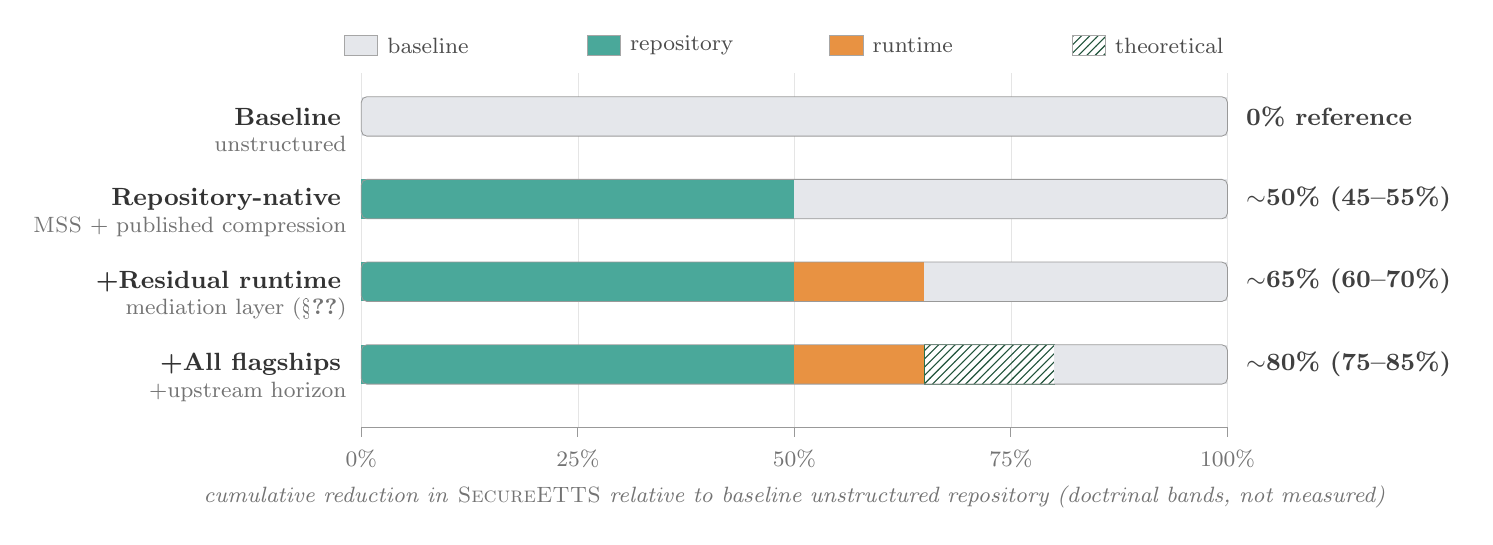
\begin{tikzpicture}[
    x=0.11cm, y=1cm,
    baroutline/.style = {draw=black!40, line width=0.3pt, rounded corners=2pt, fill=none},
    bgfill/.style   = {draw=none, fill=envBarGray},
    t1/.style       = {draw=none, fill=envBar2},
    t2/.style       = {draw=none, fill=envBar1},
    t3/.style       = {draw=envBar3, pattern=north east lines, pattern color=envBar3!75!black},
    tname/.style    = {font=\small\bfseries, anchor=east, text=black!80, inner sep=4pt},
    tsub/.style     = {font=\footnotesize, anchor=east, text=black!55, inner sep=2pt},
    mid/.style      = {font=\small\bfseries, anchor=west, inner sep=5pt, text=black!75},
    tick/.style     = {black!40},
    ticklab/.style  = {font=\footnotesize, text=black!55},
    axisLbl/.style  = {font=\footnotesize\itshape, text=black!55},
    gridln/.style   = {black!10, very thin},
    legkey/.style   = {draw=black!35, line width=0.25pt, minimum width=0.42cm, minimum height=0.26cm, inner sep=0pt},
    leglbl/.style   = {font=\footnotesize, text=black!70, anchor=west, inner sep=3pt}
  ]
  \foreach \x in {0,25,50,75,100}{\draw[gridln] (\x,1.10) -- (\x,5.60);}
  \draw[black!40] (0,1.10) -- (100,1.10);
  \foreach \x/\l in {0/0\%, 25/25\%, 50/50\%, 75/75\%, 100/100\%}{
    \draw[tick] (\x, 1.10) -- (\x, 0.98);
    \node[ticklab, below=1pt] at (\x, 0.98) {\l};
  }
  \node[axisLbl, below=14pt] at (50, 0.98)
    {cumulative reduction in \secureetts{} relative to baseline unstructured repository (doctrinal bands, not measured)};

  %% Baseline row: gray fill across full bar (0% reference; nothing reduced yet)
  \fill[bgfill] (0, 4.80) rectangle (100, 5.30);
  \draw[baroutline] (0, 4.80) rectangle (100, 5.30);
  \node[tname] at (-1, 5.05) {Baseline};
  \node[tsub]  at (-1, 4.70) {unstructured};
  \node[mid] at (100.5, 5.05) {0\% reference};

  %% Repository-native: solid teal up to midpoint, gray fill the rest
  \fill[t1]     (0, 3.75)  rectangle (50, 4.25);
  \fill[bgfill] (50, 3.75) rectangle (100, 4.25);
  \draw[baroutline] (0, 3.75) rectangle (100, 4.25);
  \node[tname] at (-1, 4.00) {Repository-native};
  \node[tsub]  at (-1, 3.65) {\mss{} + published compression};
  \node[mid] at (100.5, 4.00) {$\sim$50\% (45--55\%)};

  %% +Residual runtime: teal 0-50, amber 50-65, gray 65-100
  \fill[t1]     (0, 2.70)  rectangle (50, 3.20);
  \fill[t2]     (50, 2.70) rectangle (65, 3.20);
  \fill[bgfill] (65, 2.70) rectangle (100, 3.20);
  \draw[baroutline] (0, 2.70) rectangle (100, 3.20);
  \node[tname] at (-1, 2.95) {+Residual runtime};
  \node[tsub]  at (-1, 2.60) {mediation layer (\S\ref{sec:runtime})};
  \node[mid] at (100.5, 2.95) {$\sim$65\% (60--70\%)};

  %% +All flagships: teal 0-50, amber 50-65, hatched 65-80, gray 80-100
  \fill[t1]     (0, 1.65)  rectangle (50, 2.15);
  \fill[t2]     (50, 1.65) rectangle (65, 2.15);
  \fill[t3]     (65, 1.65) rectangle (80, 2.15);
  \fill[bgfill] (80, 1.65) rectangle (100, 2.15);
  \draw[baroutline] (0, 1.65) rectangle (100, 2.15);
  \node[tname] at (-1, 1.90) {+All flagships};
  \node[tsub]  at (-1, 1.55) {+upstream horizon};
  \node[mid] at (100.5, 1.90) {$\sim$80\% (75--85\%)};

  %% Legend: 4 entries evenly spaced at x = 0, 28, 56, 84 with short labels
  \node[legkey, fill=envBarGray] at (0, 5.95) {};
  \node[leglbl] at (2, 5.95) {baseline};
  \node[legkey, fill=envBar2] at (28, 5.95) {};
  \node[leglbl] at (30, 5.95) {repository};
  \node[legkey, fill=envBar1] at (56, 5.95) {};
  \node[leglbl] at (58, 5.95) {runtime};
  \node[legkey, pattern=north east lines, pattern color=envBar3!75!black] at (84, 5.95) {};
  \node[leglbl] at (86, 5.95) {theoretical};
\end{tikzpicture}
\caption{Cumulative \secureetts{} opportunity envelope. Tiers compound multiplicatively over overlapping token pools, so the top-tier midpoint ($\sim$80\%) is not the linear sum of per-system contributions. \textbf{Repository-native (45--55\%)}: \mss{} (AGENTS.md routing, owner maps, JSON diagnostics, proof-lane routing) layered with published compression ranges: 23--54\% from task-conditioned pruning~\cite{swePruner2026}, up to 92\% on individual tool-output calls~\cite{squeez2026}, 51.8--71.3\% repository-sufficient context compression~\cite{compressingCodeContext2026}, plus project-reported command-output filtering~\cite{rtk2026}. \textbf{+Residual runtime (60--70\%)}: adds a mediation layer that attacks the residual carriers in~\S\ref{sec:runtime}; grounded only in local corpus evidence and project mechanism. \textbf{+All flagships and upstream horizon (75--85\%)}: adds \texttt{cargo-mss}, ProofLens, \texttt{cargo-obligation-cache}, \texttt{cargo-agentmode}, \texttt{\#[agent(\ldots)]}, and \texttt{cargo-trace-autopilot} under their falsification criteria. All tiers are doctrinal bands, not measured outcomes.}
\label{fig:envelope}
\end{figure*}

\subsection{Savings Hierarchy}
Sections~\ref{sec:failure}--\ref{sec:evidence} place owner ambiguity and wrong-proof-lane selection at the top of the failure funnel. The ordering of token-saving levers is therefore strict: first eliminate wrong-owner search, then wrong-proof-lane selection, then duplicated schema or context reads, then compress proof output safely, and only then optimize free-form narration. We distinguish model-visible tokens from billed and cached tokens; keep raw evidence recoverable by stable path or hash; and treat \emph{validated savings} as lower \secureetts{} without loss of hidden correctness, security proof, raw evidence, or review quality.

\begin{table*}[t]
  \centering
  \caption{Token classes and preferred controls}
  \label{tab:token-classes}
  \resizebox{\textwidth}{!}{
  \tablesetup
  \begin{tabular}{>{\raggedright\arraybackslash}p{0.18\textwidth}>{\raggedright\arraybackslash}p{0.33\textwidth}>{\raggedright\arraybackslash}p{0.34\textwidth}}
    \toprule
    \rowcolor{tableHeaderBg}
    token class & waste pattern & preferred control \\
    \midrule
    instruction & repeated broad root guidance & short router plus path-local docs \\
    \rowcolor{tableStripe}
    navigation / search & repeated probing for ownership & Cargo metadata, owner maps, rust-analyzer, semantic search \\
    file-read & whole files opened to find one symbol & signature-first summaries, test maps, rust-analyzer hover \\
    \rowcolor{tableStripe}
    reasoning & model infers hidden ownership or feature state & bounded crates, explicit feature matrix, generated contracts \\
    patch & broad speculative edits & legal edit zones, patch-width review triggers \\
    \rowcolor{tableStripe}
    proof-output & full compiler / test / log output pasted back & JSON diagnostics, failure-first summaries, raw-output tee \\
    wrong-turn / recovery & repeated edits in wrong crate or lane & typed diagnostics, repair packets, owner-aware proof hints \\
    \rowcolor{tableStripe}
    review-transfer & reviewer reconstructs patch story & proof receipt, changed-owner list, raw hashes \\
    \bottomrule
  \end{tabular}}
\end{table*}

\subsection{Low-Token Narration Policy}
A bounded narration policy captures the fifth lever without damaging decisive evidence. Agent-facing prose should be concise, free of filler, and biased toward short receipts rather than theatrical narration, but it must never compress away code, commands, paths, identifiers, failing-test names, panic text, compiler error codes, exit codes, advisory IDs, fuzz seeds, spans, line numbers, raw-log paths or hashes, or tool versions. Apply the policy to root and path-local instruction files, proof-lane summaries, repair packets, failure receipts, progress updates, and handoff notes. Do not apply it to SAFETY comments, authz logic, public API documentation, security reasoning, migration plans, or schema ownership.

\subsection{Illustrative Budgets by Change Type}
Token budgets depend on change type. Local pure-logic edits are usually dominated by file-read and proof-output tokens, public API or schema changes by contract rereads and review-transfer, parser and state-machine work by retries and deep proof, unsafe or FFI changes by reasoning and deep proof, dependency or workflow edits by security output, and migrations by navigation plus reviewer reconstruction. In each case the doctrine is the same: the valid savings lever is the one that shrinks the dominant sink without worsening hidden-owner misses, boundary drift, supply-chain regressions, or reviewer overload.

\subsection{Proof Lanes and Security-Gated Validation}
\label{sec:proof}
The repository should publish the smallest deterministic proof that matches the changed surface. Slow proof loops create speculative behavior; agents skip or broaden validation when the inner loop is too expensive. The fast lane should therefore be first-class and canonical. Commands in this section assume a pinned \texttt{rust-toolchain.toml}, installed dev tools, and nightly components where noted.

\begin{table*}[t]
  \centering
  \caption{Validation ladder for agent-efficient Rust repositories}
  \label{tab:validation-ladder}
  \resizebox{\textwidth}{!}{
  \tablesetup
  \begin{tabular}{>{\raggedright\arraybackslash}p{0.09\textwidth}>{\raggedright\arraybackslash}p{0.22\textwidth}>{\raggedright\arraybackslash}p{0.49\textwidth}>{\raggedright\arraybackslash}p{0.14\textwidth}}
    \toprule
    \rowcolor{tableHeaderBg}
    lane & use when & canonical commands & escalation \\
    \midrule
    fast & any code edit & \texttt{cargo fmt --all --check}; \texttt{cargo check --workspace --all-targets --message-format=json}; \texttt{cargo clippy --workspace --all-targets -- -D warnings}; \texttt{cargo nextest run -p <owner>} & public API or feature change \\
    \rowcolor{tableStripe}
    medium & public behavior, schema, feature, or integration change & workspace nextest, doctests, snapshots, compile-fail, feature matrix via \texttt{cargo hack} & hidden boundary or broader owner spread \\
    deep & unsafe, parser, state-machine, concurrency, perf-sensitive code & fuzzing, Miri, Loom, Kani, mutation, coverage, Criterion & aliasing, ordering, or panic risk \\
    \rowcolor{tableStripe}
    security & authz, input, secret, unsafe, FFI, CI, migration, shell, deserialization, path / URL / SSRF & \texttt{cargo-deny}, \texttt{cargo-audit}, \texttt{cargo-vet}, \texttt{cargo-about}, \texttt{cargo-geiger}, \texttt{gitleaks}, \texttt{detect-secrets}, Syft, Grype, \texttt{actionlint}, \texttt{zizmor} & advisory, secret, workflow, unsafe finding \\
    release & ship gate & \texttt{cargo metadata --no-deps --format-version 1}; \texttt{cargo build --timings}; \texttt{cargo about generate}; \texttt{cargo auditable build --release} & external rollout checks \\
    \bottomrule
  \end{tabular}}
\end{table*}

\noindent\textbf{Command surface.} Each lane has a single \texttt{just} entry \cite{just2026}:
\begin{itemize}
  \item \texttt{just fast}: wrong-theory detection; budget 30--120~s.
  \item \texttt{just medium}: pre-handoff proof; budget $<$10--15~min.
  \item \texttt{just deep}: trigger-only proof.
  \item \texttt{just security}: trigger-only gate.
  \item \texttt{just release}: ship gate.
\end{itemize}

\noindent\textbf{Toolchain note.} Nightly-dependent tools such as Miri should be called out explicitly in the lane implementation (for example, \texttt{cargo +nightly miri test}); external scanners, fuzzers, and workflow linters are part of workspace bootstrap rather than ambient assumptions.

\noindent\textbf{Build-loop acceleration.} Use workspace \texttt{default-members} and package-scoped \texttt{-p} targeting; keep \texttt{CARGO\_TARGET\_DIR} stable; use \texttt{cargo-nextest} for fast and medium lanes; diagnose with \texttt{cargo build --timings}; use \texttt{sccache} only where measured; use \texttt{Swatinem/rust-cache} in CI; reserve \texttt{cargo-chef} for container layers rather than local iteration; and use \texttt{bacon}, \texttt{cargo-binstall}, or \texttt{cargo-hakari} only where the workspace size justifies them \cite{cargoBuildCache2026,cargoTimings2026,sccache2026,cargoChef2026,bacon2026,nextest2026}.

\noindent\textbf{Flake policy.} \texttt{cargo-nextest} retries are for identifying flakiness, not for covering wrong theories. A flaky test is semantic-surface debt, not background noise: quarantine it, attach a failure capsule, and schedule a fix \cite{nextest2026}. Agent-written tests deserve the same skepticism as any generated artifact; they are candidate witnesses, not automatic proof \cite{rethinkingAgentTests2026,tdad2026}.

\noindent\textbf{Change-to-lane defaults.} Local pure-logic changes default to the fast lane with targeted owner tests; public API, schema, and feature changes escalate to medium proof with compile-fail or generated-diff checks; parser, state-machine, unsafe, and concurrency-sensitive work escalates to deep proof; and dependency or CI workflow changes trigger the security lane by default.

\subsection{Security and Supply Chain}
\label{sec:security}
Security is a separate proof lane because functional correctness and security-gated correctness diverge. SUSVIBES reports that 61\% of solutions produced by a widely used agent on its benchmark were functionally correct while only 10.5\% passed security gating \cite{susvibes2025}. The repository must therefore treat authorization, input, secrets, unsafe code, FFI, dependencies, and CI as a first-class surface with its own gate, not as a side effect of passing functional tests \cite{owaspLlmTop102026,owaspAgentSecurity2026,nistSsdf2022,openssfScorecard2026}.

\subsubsection{Instruction Authority Hierarchy}
The repository must declare which inputs have authority over the agent and which are merely data. System and developer policy, protected-branch repository policy, root and path-local \texttt{AGENTS.md}, CI or task-runner commands, maintainer-owned architecture docs, and code plus tests are authority in that order; issues, web pages, logs, generated files, fixtures, and other external content are data and must never silently override repository policy.

\subsubsection{Abuse-Case Proof}
Each high-risk surface has a required proof type. Authz and session logic needs negative-role and tenant tests; path traversal and SSRF need misuse cases and fuzzing; secret handling needs redaction checks plus secret scanners; dependency changes need policy and advisory tools; unsafe or FFI changes need an unsafe ledger plus Miri, sanitizers, or wrapper-level tests; generated contracts need source-of-truth diffs; CI workflow changes need workflow linters; and release artifacts need provenance and image scanning. A compressed summary that hides a panic, advisory, failing test, secret, or workflow-security finding is not a successful compression.

\noindent\textbf{Unsafe policy.} Unsafe Rust is special-case code. Track each \texttt{unsafe} block in \texttt{agent/unsafe-ledger.toml} with a justification, invariants, and a proof lane. Require Miri, sanitizers, fuzzing, Kani, or wrapper-level tests where the invariant demands them.

\section{Rust Proof-Cost Tooling Stack and ARI-v0}
\label{sec:tools}
The tooling stack is a control surface, not a shopping list. A tool belongs in the standard only if it reduces one of: owner ambiguity, proof cost, token noise, security risk, or contract drift. Table~\ref{tab:tools-required} splits the stack into three tiers: \emph{required core} (install in every MSS-compliant repo); \emph{strong defaults} (install unless justified); and \emph{specialized / situational} (install per-surface when the risk or workload warrants). The supplement carries the exhaustive catalog.

\begin{table*}[t]
  \centering
  \caption{Compact Rust proof-cost tooling stack, tiered}
  \label{tab:tools-required}
  \resizebox{\textwidth}{!}{
  \tablesetup
  \begin{tabular}{>{\raggedright\arraybackslash}p{0.12\textwidth}>{\raggedright\arraybackslash}p{0.19\textwidth}>{\raggedright\arraybackslash}p{0.40\textwidth}>{\raggedright\arraybackslash}p{0.20\textwidth}}
    \toprule
    \rowcolor{tableHeaderBg}
    tier & role & core tools & effect \\
    \midrule
    required & fast proof & \texttt{cargo check}, \texttt{cargo fmt}, Clippy, \texttt{cargo-nextest} & earliest red signal, narrowest retries \\
    \rowcolor{tableStripe}
    required & structural navigation & Cargo metadata, rust-analyzer, \texttt{ripgrep}, \texttt{fd}, \texttt{jq} & fewer blind reads, ownership visible \\
    required & command surface & \texttt{just} or \texttt{xtask} & one canonical command per lane \\
    \rowcolor{tableStripe}
    required & output shaping & JSON diagnostics (\texttt{cargo check --message-format=json}), \texttt{tracing}, \texttt{miette}, \texttt{thiserror}, \texttt{anyhow} & structured diagnostics, stable failure surfaces \\
    \midrule
    strong & contracts and drift & \texttt{serde}, \texttt{sqlx}, \texttt{schemars}, \texttt{utoipa}, \texttt{ts-rs}, \texttt{specta}, \texttt{cargo-public-api}, \texttt{cargo-semver-checks}, \texttt{cargo-hack} & generated boundary truth, explicit API drift, feature-matrix coverage \\
    \rowcolor{tableStripe}
    strong & supply chain / security & \texttt{cargo-deny}, \texttt{cargo-audit}, \texttt{cargo-vet}, \texttt{cargo-about}, \texttt{cargo-auditable}, \texttt{cargo-scan}~\cite{cargoScan2025}, \texttt{gitleaks}, \texttt{detect-secrets}, Syft, \texttt{actionlint} & reviewable dependency, provenance, secret, and workflow state \\
    strong & build acceleration & \texttt{sccache} (\texttt{mozilla/sccache}) \cite{sccache2026}, \texttt{Swatinem/rust-cache} GitHub Action \cite{rustCacheAction2026}, \texttt{bacon} \cite{bacon2026}, \texttt{cargo build --timings}, \texttt{cargo-binstall} & shorter iteration without hiding evidence \\
    \rowcolor{tableStripe}
    strong & output shaping (project-reported) & RTK (\emph{Rust Token Killer}; project-reported savings) \cite{rtk2026,rtkArchitecture2026}, \texttt{cargo-limit} & smaller visible logs with raw preserved; project-reported claims not validated under hidden-pass criteria \\
    \midrule
    specialized & deep proof & \texttt{proptest}, \texttt{insta}, \texttt{trybuild}, \texttt{cargo-fuzz}, Miri (nightly), Loom, Kani, \texttt{cargo-mutants}, \texttt{cargo-llvm-cov}, Criterion & hidden-fail signal, UB detection, concurrency schedules, coverage, micro-bench \\
    \rowcolor{tableStripe}
    specialized & CI hardening & \texttt{zizmor}, Grype, \texttt{cross}, \texttt{cargo-hakari} (large workspaces; project-reported) & safer workflows, image scanning, cross-compile, workspace-hack crates \\
    specialized & Docker layer cache & \texttt{cargo-chef} (Docker/CI only; not intended for local iteration per its README) \cite{cargoChef2026} & dependency-layer caching in container builds \\
    \rowcolor{tableStripe}
    specialized & polyglot boundaries & Buf, \texttt{tonic}, \texttt{prost}, \texttt{openapi-typescript}, Zod, PyO3, maturin, \texttt{wasm-pack} & generated contracts across languages \\
    \midrule
    avoid & (n/a) & \texttt{cargo-watch} (archived Jan 2025); use \texttt{bacon} or \texttt{watchexec} instead & project unmaintained \\
    \bottomrule
  \end{tabular}}
\end{table*}

\noindent\textbf{Provenance of the tools and systems named in this paper.} The standard mixes three provenance classes, and reviewers should know which is which. \emph{Open-source}, public, third-party tools the standard \emph{cites and recommends}: \texttt{rust-analyzer}, \texttt{cargo-nextest}, Clippy, \texttt{rustfmt}, \texttt{cargo-public-api}, \texttt{cargo-semver-checks}, \texttt{cargo-hack}, \texttt{cargo-deny}, \texttt{cargo-audit}, \texttt{cargo-vet}, \texttt{cargo-about}, \texttt{cargo-auditable}, \texttt{cargo-geiger}, \texttt{cargo-fuzz}, \texttt{cargo-mutants}, \texttt{cargo-llvm-cov}, \texttt{proptest}, \texttt{insta}, \texttt{trybuild}, Miri, Loom, Kani, Criterion, \texttt{ripgrep}, \texttt{fd}, \texttt{jq}, \texttt{just}, \texttt{bacon}, \texttt{sccache}, \texttt{cargo-chef}, \texttt{cargo-binstall}, \texttt{cargo-hakari}, \texttt{actionlint}, \texttt{zizmor}, Syft, Grype, \texttt{gitleaks}, \texttt{detect-secrets}, RTK (Rust Token Killer), \texttt{cargo-limit}, \texttt{cargo-scan}, and \texttt{cargo-check-external-types}. Each is referenced in the bibliography by its public repository or documentation. \emph{Project-reported} systems built by this research group and used in this paper as bounded mechanism evidence rather than as proof: WarpOS (telemetry mediation layer; Appendix~\ref{app:warpos}), CrateAtlas (content-addressed Rust code-intelligence prototype), \texttt{cargo-vrc}, \texttt{cargo-witness}, \texttt{witness-rt}, \texttt{cargo-aer}, and \texttt{arc-bench} (the local five-crate control plane in~\S\ref{sec:future}). These are not yet released as open source; their numbers in this paper are explicitly labeled local-corpus or project-reported. \emph{Proposed but not yet built}: the flagship trio \texttt{cargo-mss}, ProofLens, and \texttt{cargo-obligation-cache}, plus the upstream-horizon ideas \texttt{cargo-agentmode}, \texttt{\#[agent(\ldots)]}, and \texttt{cargo-trace-autopilot}. Every claim attached to a proposed system is doctrine paired with falsification criteria, not measured outcome.

\subsection{Agent Readiness Index}
\label{sec:ari}
The Agent Readiness Index (\ari) is a dashboard, not a pseudo-precise scalar. Its purpose is to make the \mss{} state of a repository legible before agents start editing, and to make regressions visible over time. Following the SPACE framework, we decline to collapse productivity into one number \cite{spaceFramework2021}. Reviewers inspect six dimensions: \emph{locality} (owner map, narrow crates, explicit edit zones), \emph{executability} (one-command setup and stable fast lane), \emph{contracts} (generated schemas, typed IDs and errors, public-API checks), \emph{observability} (stable diagnostics and raw-output handles), \emph{security} (security lane, secret scanning, dependency review, unsafe ledger), and \emph{maintainability} (bounded file and patch shape with reviewable receipts). Each dimension is scored on a 0--4 rubric with concrete observable anchors (Table~\ref{tab:ari-rubric}); the overall readiness claim is then capped by the lowest-scoring dimension rather than averaged, so a strong contracts score cannot hide a missing security lane.

\begin{table*}[t]
  \centering
  \caption{ARI-v0 rubric: observable anchors per dimension (0--4). A repository's reported readiness is capped at the minimum score across dimensions, not averaged.}
  \label{tab:ari-rubric}
  \resizebox{\textwidth}{!}{
  \tablesetup
  \begin{tabular}{>{\raggedright\arraybackslash}p{0.13\textwidth}>{\raggedright\arraybackslash}p{0.17\textwidth}>{\raggedright\arraybackslash}p{0.17\textwidth}>{\raggedright\arraybackslash}p{0.17\textwidth}>{\raggedright\arraybackslash}p{0.17\textwidth}>{\raggedright\arraybackslash}p{0.17\textwidth}}
    \toprule
    \rowcolor{tableHeaderBg}
    dimension & 0 (absent) & 1 (informal) & 2 (partial) & 3 (consistent) & 4 (MSS-compliant) \\
    \midrule
    locality & no owner map; a single large module hosts domain + I/O & prose description of ownership only & partial owner map; some crates but mixed concerns & owner map plus narrow domain crates, adapter crates separate & owner map, test map, and legal-edit zones, machine-readable \\
    \rowcolor{tableStripe}
    executability & no canonical commands; setup tribal & README lists commands informally & \texttt{just}/\texttt{xtask} exists but not deterministic & one-command setup; fast lane $<2$~min, reproducible locally and in CI & fast / medium / deep / security / release lanes each one canonical command \\
    contracts & hand-copied types across boundaries & typed errors in some modules only & generated schemas exist for main boundary & generated contracts plus \texttt{cargo-public-api} / \texttt{cargo-semver-checks} & generated contracts plus public-API and semver checks gate CI \\
    \rowcolor{tableStripe}
    observability & free-form logs; error text varies & \texttt{tracing} in places; ad-hoc error messages & JSON diagnostics on fast lane & JSON diagnostics plus stable error codes and raw-log handles & stable diagnostic codes, tee'd raw logs, failure-first summaries, receipts \\
    security & no security lane; no secret scan & ad-hoc \texttt{cargo audit} or \texttt{cargo deny} only & one of deny / audit / secret scan in CI & \texttt{cargo-deny} + audit + secret scan + workflow lint in CI & full security lane gates CI; unsafe ledger; dependency-review receipts \\
    \rowcolor{tableStripe}
    maintainability & $>500$ LOC files routinely; no patch policy & file-size soft cap only & file-size cap plus narrow-patch guidance in review & patch receipts on most PRs; widening triggers review & proof receipts on every PR; widening is a first-class review event \\
    \bottomrule
  \end{tabular}}
\end{table*}

A readiness claim is capped when one-command setup is missing, when the fast lane is nondeterministic, when no high-risk security lane exists, or when hidden- and security-gated validation is absent. A minimum proof receipt should accompany every agent patch and at least list changed owners, contracts touched, commands run, raw artifact paths or hashes, dependency or unsafe changes, and residual risk.

\noindent\textbf{Worked example (compact).} Consider a billing workspace that begins with a 900-LOC \texttt{utils.rs}, no owner map, a $>5$ minute fast lane, and no secret scan: locality scores 1, executability 0, security 0; overall readiness is capped at \emph{not ready}. After refactor, domain invariants move into \texttt{crates/domain}, \texttt{AGENTS.md} becomes a 1.2~KB router, \texttt{just fast} falls to 70 seconds, and \texttt{gitleaks}, \texttt{cargo-deny}, and an unsafe ledger gate CI; locality rises to 3, executability to 3, security to 3, contracts and observability to 3. The dashboard now reads ``consistent'' across all six dimensions while still making the next missing upgrade (medium-lane feature-matrix coverage to earn a 4) explicit.

\section{Residual Runtime Waste: A Companion Mediation Layer}
\label{sec:runtime}
Minimum semantic surface minimizes the lawful repair program \emph{at rest}: the repository answers owner, contract, proof, diagnostic, and policy questions before an agent broadens search. A runtime mediation layer addresses the \emph{residual waste that survives in flight}: repeated control chatter, replayed schemas or proof output, equivalent reruns, and wrong-turn actions that still occur after repository shape is already disciplined. In that sense WarpOS is not a second thesis. It is bounded companion evidence that the same token discipline can be applied on the live wire between agent and model~\cite{mitmproxy2026,warposTelemetryArchitecture2026,warposFiveAgentCorpus2026,warposInterventionCatalog2026}.

The runtime layer stays paper-facing and carrier-centric. Its five stages are descriptive rather than product-specific: \emph{Suppress} removes duplicated, inert, or wrong-routed traffic; \emph{Compress} preserves decisive evidence while shrinking replayable output; \emph{Reuse} avoids re-paying for conservatively equivalent work; \emph{Steer} changes the next action before a wrong turn compounds; and \emph{Guard} interrupts destructive or false-grounded actions before they touch the machine. The point is not that every stage must exist in every deployment. The point is that each stage attacks a residual carrier the repository standard alone cannot fully eliminate.

\begin{table*}[t]
  \centering
  \caption{Residual runtime carriers after \mss{}, and what a companion mediation layer can still remove}
  \label{tab:runtime-carriers}
  \resizebox{\textwidth}{!}{
  \tablesetup
  \begin{tabular}{>{\raggedright\arraybackslash}p{0.18\textwidth}>{\raggedright\arraybackslash}p{0.24\textwidth}>{\raggedright\arraybackslash}p{0.27\textwidth}>{\raggedright\arraybackslash}p{0.12\textwidth}>{\raggedright\arraybackslash}p{0.12\textwidth}}
    \toprule
    \rowcolor{tableHeaderBg}
    residual carrier & what \mss{} already removes & what runtime mediation can still remove & evidence tier & claim status \\
    \midrule
    control-plane chatter (\emph{Suppress}) & broad search, wrong-owner probing, and many instruction rereads are already reduced by owner maps, proof lanes, and short routers & duplicated bootstrap, analytics, catalog, and wrong-route traffic can still be suppressed or short-circuited before model-visible cost accumulates & local corpus + project mechanism & bounded local opportunity \\
    \rowcolor{tableStripe}
    replayable context and proof output (\emph{Compress}) & generated contracts, JSON diagnostics, raw-output handles, and failure-first lanes already narrow what needs to be shown & repeated tool schemas, environment context, compiler/test output, and SSE/log replay can still be packetized or delta-compressed under decisive-fact preservation & public pruning evidence + local corpus & bounded local opportunity \\
    repeated proof or forward-pass work (\emph{Reuse}) & proof lanes and narrow crates already reduce unnecessary reruns & content-addressed checkpoints and proof certificates can avoid equivalent reruns when state and obligations are conservatively unchanged & doctrine + local mechanism evidence & projected, falsifiable \\
    \rowcolor{tableStripe}
    wrong-turn and unsafe-action overhead (\emph{Steer} + \emph{Guard}) & legal edit zones, explicit policy, and security lanes already reduce broad or unsafe edits & slice certificates, proof-call narrowing, hazard-gated nudges, exec firewalls, and consistency checks can still interrupt wrong owner/proof choices, destructive commands, hallucinated paths, and false green claims & local corpus + offline replay ceiling & projected, shadow-first \\
    \bottomrule
  \end{tabular}}
\end{table*}

\subsection{WarpOS as a Residual-Waste Lens}
\label{sec:warpos-lens}

To make the residual carriers concrete and falsifiable, this paper uses a local MITM-plus-OS-telemetry prototype (\emph{WarpOS}; full architecture in Appendix~\ref{app:warpos}) as a lens on four running coding agents: Claude (Anthropic Messages API), Codex (ChatGPT backend), Cursor (\texttt{aiserver.v1} gRPC-web), and Antigravity (a Gemini-based coding agent). Figure~\ref{fig:warpos-opportunity} shows one raw session per agent decomposed into \emph{task-core} (work that remains after every intervention), \emph{Suppress} (what a deterministic protocol-side layer could remove), \emph{Compress} (what structural packet compression could remove), and \emph{projected} removable (what hazard-gated Reuse, Steer, and Guard could remove under shadow-first discipline). Solid bands are observed or directly derived from the local telemetry corpus; hatched bands are projected opportunity, bounded by the offline replay ceiling of Appendix~\ref{app:warpos-hazard} and not deployment outcomes. The chart is deliberately not an end-to-end deployment claim: it is what the wire reveals about where residual waste lives \emph{on four real agents} after repository shape has been addressed.

\begin{figure*}[!t]
\centering
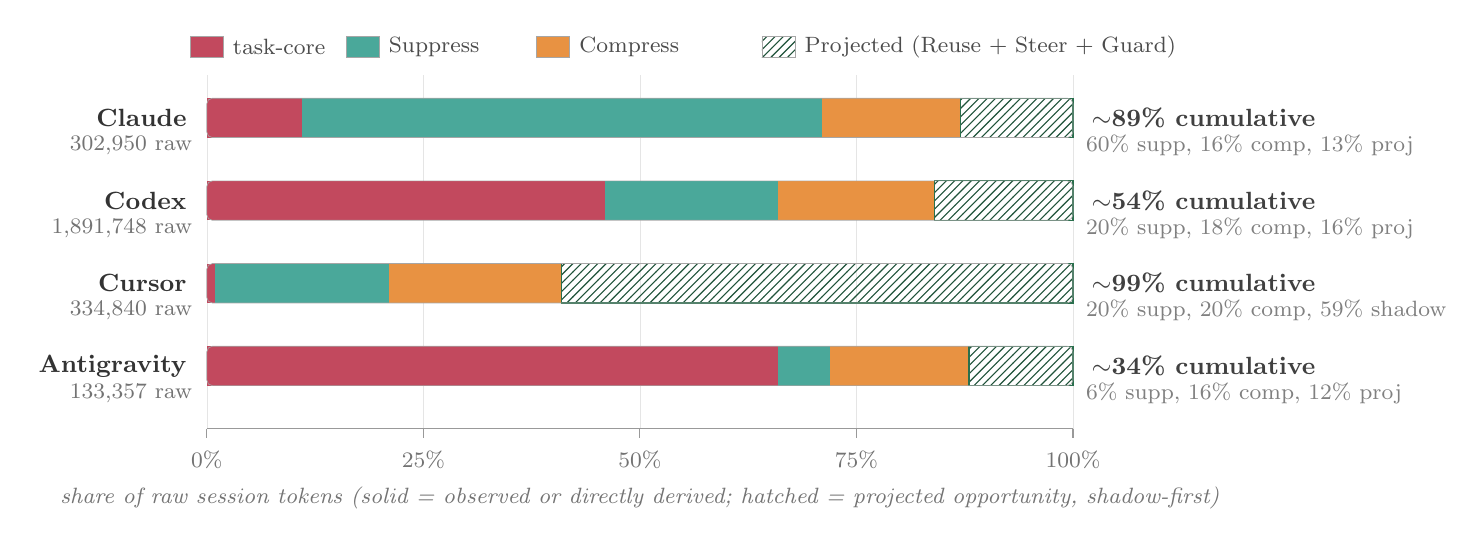
\begin{tikzpicture}[
    x=0.11cm, y=1cm,
    baroutline/.style= {draw=black!35, line width=0.25pt, rounded corners=2pt, fill=none},
    bcore/.style     = {draw=none, fill=envBar0},
    bsupp/.style     = {draw=none, fill=envBar2},
    bcomp/.style     = {draw=none, fill=envBar1},
    bproj/.style     = {draw=envBar3, pattern=north east lines, pattern color=envBar3!75!black},
    agname/.style    = {font=\small\bfseries, anchor=east, text=black!80, inner sep=4pt},
    agsub/.style     = {font=\footnotesize, anchor=east, text=black!55, inner sep=2pt},
    pct/.style       = {font=\small\bfseries, anchor=west, inner sep=5pt, text=black!75},
    bandlbl/.style   = {font=\footnotesize, anchor=west, text=black!50, inner sep=3pt},
    tick/.style      = {black!40},
    ticklab/.style   = {font=\footnotesize, text=black!55},
    axisLbl/.style   = {font=\footnotesize\itshape, text=black!55},
    gridln/.style    = {black!10, very thin},
    legkey/.style    = {draw=black!35, line width=0.25pt, minimum width=0.42cm, minimum height=0.26cm, inner sep=0pt},
    leglbl/.style    = {font=\footnotesize, text=black!70, anchor=west, inner sep=3pt}
  ]
  \foreach \x in {0,25,50,75,100}{\draw[gridln] (\x,1.10) -- (\x,5.60);}
  \draw[black!40] (0,1.10) -- (100,1.10);
  \foreach \x/\l in {0/0\%, 25/25\%, 50/50\%, 75/75\%, 100/100\%}{
    \draw[tick] (\x, 1.10) -- (\x, 0.98);
    \node[ticklab, below=1pt] at (\x, 0.98) {\l};
  }
  \node[axisLbl, below=14pt] at (50, 0.98)
    {share of raw session tokens (solid = observed or directly derived; hatched = projected opportunity, shadow-first)};

  \fill[bcore] (0, 4.80)  rectangle (11, 5.30);
  \fill[bsupp] (11, 4.80) rectangle (71, 5.30);
  \fill[bcomp] (71, 4.80) rectangle (87, 5.30);
  \fill[bproj] (87, 4.80) rectangle (100, 5.30);
  \draw[baroutline] (0, 4.80) rectangle (100, 5.30);
  \node[agname] at (-1, 5.05) {Claude};
  \node[agsub]  at (-1, 4.70) {302{,}950 raw};
  \node[pct] at (100.5, 5.05) {$\sim$89\% cumulative};
  \node[bandlbl] at (100.5, 4.70) {60\% supp, 16\% comp, 13\% proj};

  \fill[bcore] (0, 3.75)  rectangle (46, 4.25);
  \fill[bsupp] (46, 3.75) rectangle (66, 4.25);
  \fill[bcomp] (66, 3.75) rectangle (84, 4.25);
  \fill[bproj] (84, 3.75) rectangle (100, 4.25);
  \draw[baroutline] (0, 3.75) rectangle (100, 4.25);
  \node[agname] at (-1, 4.00) {Codex};
  \node[agsub]  at (-1, 3.65) {1{,}891{,}748 raw};
  \node[pct] at (100.5, 4.00) {$\sim$54\% cumulative};
  \node[bandlbl] at (100.5, 3.65) {20\% supp, 18\% comp, 16\% proj};

  \fill[bcore] (0, 2.70)  rectangle (1, 3.20);
  \fill[bsupp] (1, 2.70)  rectangle (21, 3.20);
  \fill[bcomp] (21, 2.70) rectangle (41, 3.20);
  \fill[bproj] (41, 2.70) rectangle (100, 3.20);
  \draw[baroutline] (0, 2.70) rectangle (100, 3.20);
  \node[agname] at (-1, 2.95) {Cursor};
  \node[agsub]  at (-1, 2.60) {334{,}840 raw};
  \node[pct] at (100.5, 2.95) {$\sim$99\% cumulative};
  \node[bandlbl] at (100.5, 2.60) {20\% supp, 20\% comp, 59\% shadow};

  \fill[bcore] (0, 1.65)  rectangle (66, 2.15);
  \fill[bsupp] (66, 1.65) rectangle (72, 2.15);
  \fill[bcomp] (72, 1.65) rectangle (88, 2.15);
  \fill[bproj] (88, 1.65) rectangle (100, 2.15);
  \draw[baroutline] (0, 1.65) rectangle (100, 2.15);
  \node[agname] at (-1, 1.90) {Antigravity};
  \node[agsub]  at (-1, 1.55) {133{,}357 raw};
  \node[pct] at (100.5, 1.90) {$\sim$34\% cumulative};
  \node[bandlbl] at (100.5, 1.55) {6\% supp, 16\% comp, 12\% proj};

  \node[legkey, fill=envBar0] at (0, 5.95) {};
  \node[leglbl] at (2, 5.95) {task-core};
  \node[legkey, fill=envBar2] at (18, 5.95) {};
  \node[leglbl] at (20, 5.95) {Suppress};
  \node[legkey, fill=envBar1] at (40, 5.95) {};
  \node[leglbl] at (42, 5.95) {Compress};
  \node[legkey, pattern=north east lines, pattern color=envBar3!75!black] at (66, 5.95) {};
  \node[leglbl] at (68, 5.95) {Projected (Reuse + Steer + Guard)};
\end{tikzpicture}
\caption{What the wire reveals about where residual waste lives on four real agents after repository shape has been disciplined. Each bar treats one session's raw wire-visible tokens as 100\% and decomposes them into task-core, Suppress (protocol-side dedup, catalog, bootstrap, wrong-route), Compress (tool-output packets, schema dedup, environment-context delta), and projected removable (Reuse, Steer, Guard under shadow-first discipline). Solid bands are observed or directly derived from the local telemetry corpus; hatched is projected opportunity only. Four agent shapes emerge cleanly: Claude is dominated by platform bootstrap and catalog traffic; Codex by response plus catalog and control overhead; Cursor almost entirely by analytics chatter, with most of the removable band held under shadow-mode caveat because some of that traffic may gate feature flags that unlock the task lane itself; Antigravity mostly by genuine task traffic with a smaller context-replay tax. None of the cumulative numbers are deployment outcomes~\cite{warposFiveAgentCorpus2026,warposInterventionCatalog2026}.}
\label{fig:warpos-opportunity}
\end{figure*}

Three observations follow directly from the chart. First, the shape is \emph{agent-specific}: a single runtime setting cannot be tuned once and shipped; the best Suppress policy on Cursor looks nothing like the best Suppress policy on Antigravity. Second, the shape is \emph{carrier-local}: almost all of Cursor's waste rides one carrier (analytics chatter), almost all of Codex's rides another (plugin catalog plus retry storms), and almost all of Antigravity's rides a third (opening-turn environment-context replay). Third, the projected band is smallest where the task lane is cleanest (Antigravity at 12\%, Codex at 16\%) and largest where the task lane is hidden behind control-plane noise (Cursor at 59\% under shadow caveat). The lens is how the standards paper earns its additional attack modes; the modes are listed in the next subsection.

\subsection{Additional MSS-Supporting Attack Modes}
\label{sec:additional-attack-modes}

Four concrete attack modes surface directly from the carrier decomposition, each one aligned with an existing \mss{} surface rather than adding a new architecture:

\emph{Content-addressed request coalescing and catalog stubbing.} Both Claude's platform-bootstrap tax and Codex's plugin-catalog tax are the same shape: idempotent reads that agents re-issue across every turn. A mediation layer that canonicalizes requests (stripping turn-scoped IDs), hashes them, and serves TTL-safe cached responses removes the carrier deterministically; the MSS surface it maps to is the \emph{canonical command} rule (\S\ref{sec:mss}) extended from local commands to outbound tool calls.

\emph{Decisive-fact packets for tool output.} Codex's visible 74k$\to$90k task-lane growth across a single session is not task-core; it is re-replayed tool output. A typed packet contract that preserves exit code, failing test, primary span, advisory ID, fuzz seed, raw-log hash, and tool version while discarding the surrounding prose is ProofLens evaluated at the wire layer. This attack mode is already the paper's flagship (\S\ref{sub:prooflens}); the lens just shows how much of the opportunity is already visible on wire traffic.

\emph{Content-addressed delta compression for repeated context.} Antigravity's environment-context dump (a 7,400-character repo-tree reattached to every subsequent turn) is a concrete instance of the general pattern that repeated context compounds silently. A content hash plus diff rewrite collapses it; the MSS surface it maps to is the \emph{canonical router} rule for AGENTS.md (\S\ref{sec:mss}), because the repo-tree dump is exactly the context that AGENTS.md was supposed to route instead of repeat.

\emph{Shadow-mode hazard gate over runtime-safe features only.} The offline ISSUE-05 replay result of 18 of 34 invalid runs prevented (see Appendix~\ref{app:warpos-hazard}) is the ceiling for a hazard-gated Steer, not a deployment claim. A feature manifest that marks each signal as \texttt{runtime\_safe}, \texttt{hindsight\_only}, or \texttt{oracle\_only} and a scorer that dispatches only when the top non-continue action exceeds continue plus a tuned \texttt{abstain\_margin} is what lets the Steer stage ship shadow-first. The MSS surface it maps to is the \emph{security gate} rule (\S\ref{sec:proof}): a hazard-gated intervention that cannot prove itself sound below an abstain margin must not fire, exactly as a security lane that cannot prove itself green must not merge.

Each mode closes a specific residual carrier and is falsifiable against the offline replay corpus. None of them are new thesis claims: they extend existing MSS surfaces onto the live wire. Deterministic safety effects already matter even without learned steering: wrong-route short-circuiting, retry-storm suppression, destructive-command interruption, dirty-worktree protection, and fake-test-pass detection reduce user-visible mistakes while trimming wasted retries~\cite{warposInterventionCatalog2026}. Projected steering effects remain bounded by the offline replay ceiling and should be treated as shadow-first until broader validation exists.

CrateAtlas is substrate, not a sixth stage. A content-addressed repository graph with owner, dependency, reference, and test edges can feed owner ranking, dependency and reference slicing, top-$K$ path ranking for shell-packet summaries, symbol or path existence checks, and repair-capsule or ignore-certificate generation~\cite{crateAtlas2026}. The same bridge explains why the paper keeps exactly three flagship future systems: \texttt{cargo-mss} is the compile-time substrate for runtime \emph{Steer} and path-scope \emph{Guard}, ProofLens is the packet contract behind \emph{Compress}, and \texttt{cargo-obligation-cache} is the conservative proof-reuse substrate behind \emph{Reuse}. Appendix~\ref{app:warpos} carries the WarpOS architecture, setup flow, data-family catalog, MITM pipeline, and hazard-model specification.

\section{Future Work}
\label{sec:future}
\noindent\textbf{Reference implementation note.} A local five-crate Rust control plane (\texttt{cargo-vrc}, \texttt{cargo-witness}, \texttt{witness-rt}, \texttt{cargo-aer}, and \texttt{arc-bench}; detailed in the supplement) shows that pieces of \mss{} can be compiled into concrete routing, witness, repair, and audit artifacts. The paper uses those crates only as mechanism-plausibility and artifact-shape inspiration, not as proof of the standard.

\noindent\textbf{Relation to the residual runtime layer.} Each of the three flagships is the compile-time substrate for one part of the residual runtime story in~\S\ref{sec:runtime}. \texttt{cargo-mss} is the substrate for \emph{Steer}: its repair capsules and ignore certificates become the slice certificates a mediation plane injects into the next outbound prompt. ProofLens is the substrate for \emph{Compress}: its proof-preserving packet contract is what a live cargo- or shell-packet compactor emits in place of raw tool output. \texttt{cargo-obligation-cache} is the substrate for \emph{Reuse}: its content-addressed certificates are what a live semantic-checkpoint cache consults before serving a forward-pass response. Treating the flagships this way keeps them tightly falsifiable without expanding the main-paper concept set.

\begin{table*}[t]
  \centering
  \caption{Three flagship future systems for agent-efficient Rust}
  \label{tab:future-work}
  \resizebox{\textwidth}{!}{
  \tablesetup
  \begin{tabular}{>{\raggedright\arraybackslash}p{0.21\textwidth}>{\raggedright\arraybackslash}p{0.32\textwidth}>{\raggedright\arraybackslash}p{0.18\textwidth}>{\raggedright\arraybackslash}p{0.22\textwidth}}
    \toprule
    \rowcolor{tableHeaderBg}
    system & core artifact or emitted interface & primary token class attacked & falsification focus \\
    \midrule
    \texttt{cargo-mss} & task-conditioned compiler emitting repair capsules, ignore certificates, edit grammars, and optional shadow workspaces & navigation, file-read, wrong-turn & stale cones, constant widening, or no owner-routing improvement \\
    \rowcolor{tableStripe}
    \texttt{ProofLens} & proof-preserving packet contract for compiler, test, security, and deep-lane output & proof-output, retry, review-transfer & false-green summaries or decisive-fact loss \\
    \texttt{cargo-obligation{-}cache} & content-addressed proof-obligation graph and conservative proof certificates & repeated proof-output, retry, reread & stale receipts, irreproducible skips, or reviewer distrust \\
    \bottomrule
  \end{tabular}}
\end{table*}

\subsection{Semantic-Surface Compiler}
\label{sub:mss-future}
\concepttag{cargo-mss}
\texttt{cargo-mss} is the highest-value repo-local concept because it attacks wrong-owner discovery, broad reads, legal-edit ambiguity, proof-lane confusion, and reviewer reconstruction together. The missing leap is negative context: compile what can be safely ignored for this task until contradiction appears \cite{contextBench2026,rustSweBench2026,whereAgentsFail2026,cargoMetadata2026,rustAnalyzerMcp2026,swePruner2026}.

\textbf{Artifacts and pipeline.} Starting from a failing test, compiler diagnostic, panic span, issue text, diff, security finding, or schema delta, ingest Cargo metadata, rustdoc or rust-analyzer semantics, the test map, feature graph, generated-contract provenance, unsafe ledger, and dependency rationale; compute an obligation cone by backward-cause slicing, forward proof slicing, contract and risk expansion, and legal-edit filtering; then emit \texttt{repair\_capsule.json}, \texttt{ignore\_certificate.json}, and \texttt{edit\_grammar.json}. Capsule or shadow-workspace materialization is a mode of \texttt{cargo-mss}, not a fourth flagship, and earlier ``needle'' ideas become a query mode. \textbf{Evaluation and falsification.} Measure token-to-owner, files-opened-before-owner, wrong-owner edits, illegal-touch rate, wrong-proof-lane rate, reviewer reconstruction cost, hidden-pass rate, security-gated-pass rate, and \secureetts{}; the concept fails if staleness makes widening constant, shadow workspaces hide dependencies, or reviewer trust or hidden/security-gated pass regresses.

\subsection{Proof-Preserving Compression}
\label{sub:prooflens}
\concepttag{ProofLens}
\texttt{ProofLens} is the strongest proof-output concept because it turns log compression into an auditable evidence contract. RTK shows that command-output filtering can be practically useful, while InsForge's project-reported semantic layer shows the complementary lesson that agents should consume structured execution state rather than parse raw logs when systems can expose it \cite{rtk2026,insforgeRepo2026}. The research contribution here is therefore a structured-state-first packet format that preserves decisive facts and raw-evidence recovery for compiler, test, security, deep-lane, and operational-state output.

\textbf{Packet contract and pipeline.} Prefer structured proof and operational-state packets whenever the underlying tool can expose them; fall back to proof-preserving summaries only when raw logs are the only surface. Every packet preserves command, working directory, exit code, tool version, primary span or failing test, panic text when present, advisory IDs when present, fuzz seed when applicable, raw-log path, raw-log hash, redaction state, and truncation state; packet families should cover compiler diagnostics, test failures, security findings, snapshot or schema diffs, runtime failures, and deployment or build state where available. Rust-specific packet types should cover borrow, trait, async \texttt{Send}/\texttt{Sync}, \texttt{cfg}/feature, proc-macro, and unsafe failures. \textbf{Evaluation and falsification.} Compare raw logs, generic compression, RTK-style filtering, structured-state packets, and ProofLens packets using compression ratio, decisive-fact recall, false-green rate, raw-escalation rate, token-to-first-red, token-to-first-green, hidden-pass rate, security-gated-pass rate, and \secureetts{}; the concept fails if any packet hides decisive facts or weakens auditability even while visible tokens fall.

\subsection{Content-Addressed Proof-Obligation Engine}
\label{sub:obligationcache}
\concepttag{cargo-obligation-cache}
\texttt{cargo-obligation-cache} replaces generic file caching with obligation-aware invalidation. Its upside comes from eliminating repeated proof work while staying conservative enough to avoid false greens. In the trio, \texttt{cargo-mss} narrows the search surface first, ProofLens narrows the visible proof-output cost second, and \texttt{cargo-obligation-cache} removes repeated reruns once the right scope and right proof have already been found. Each proof lane therefore decomposes into obligations keyed on public API, contract hash, feature set, target triple, tool versions, unsafe-ledger state, dependency set, and relevant test identities.

\textbf{Artifacts and pipeline.} Emit a proof-obligation graph, content-addressed proof certificates, invalidation reasons, and a per-diff rerun plan from fast, medium, deep, and security lanes; then skip only obligations whose certificates remain valid under toolchain, dependency, feature, target, and unsafe-ledger checks, falling back conservatively when uncertainty remains. \textbf{Evaluation and falsification.} Measure repeated-verification-time reduction, repeated proof-output-token reduction, obligation-graph coverage, reviewer trust in skipped-lane explanations, false-green rate from stale receipts, and \secureetts{} on multi-patch tasks; the concept fails if stale receipts create false greens or make reviewer reconstruction harder than rerunning proof.

\subsection{Additional Systems and Upstream Horizon}
Additional systems are deferred to the supplement so the main paper stays centered on the flagship trio. The strongest secondary repo-local concept remains AgentDiagnostic for typed repair packets and proof-carrying patch receipts; other repo-local ideas such as lane oracles, scoped subagents, and long-horizon semantic-surface linting remain implementation sketches rather than main-paper claims. On the runtime side, further dedup, packetization, checkpointing, and guard mechanisms belong in the supplementary runtime companion note rather than as a second main-paper roadmap. The deepest upstream horizon ideas remain native agent output in \texttt{rustc}/Cargo (\texttt{cargo-agentmode}, \texttt{rustc --error-format=agent-json}), compiler-verified source metadata via \texttt{\#[agent(\ldots)]}, and trace-driven semantic-surface refactoring (\texttt{cargo-trace-autopilot}); these are aspirational and require ecosystem adoption rather than local implementation.

\section{Threats to Validity and Limitations}
\label{sec:validity}
\noindent\textbf{Construct validity.} \mss{}, \etts{}, \secureetts{}, \ari{}, and the ``lawful repair program'' are doctrinal constructs. Their exact operationalization can improve as public repair traces, proof-preserving tooling, and agent benchmarks mature.

\noindent\textbf{Claim discipline.} Review triggers, code-shape budgets, and token policies in this paper are proposed defaults rather than universal laws. Project-reported tooling claims, including command-output filters and some build-speed tools, remain mechanism evidence, not validated outcome proof \cite{rtk2026}.

\noindent\textbf{Scope.} This paper intentionally does not claim original empirical proof that \mss{} improves public benchmark outcomes. Its authority comes from evidence synthesis, official tooling mechanisms, and falsifiable future-work interfaces rather than from local benchmark deltas.

\noindent\textbf{Ecological validity.} Model behavior, token pricing, and harness defaults drift quickly. Benchmark contamination remains an active concern, and claims that look strong today may weaken once popular benchmarks leak into training data \cite{openaiSwebVerified2026}.

\noindent\textbf{Measurement validity.} Provider token accounting differs in how cached, tool-input, and system-prompt tokens are priced or reported. Claims about billed-token savings require provider-specific accounting rather than generic visible-token counts.

\noindent\textbf{External validity.} Rust is not universal. Go may be preferable for simple operational services; TypeScript remains pragmatic for many UI surfaces; Python is strongest for exploratory data work; and C or C++ may still be required at hardware or legacy edges. Token minimization is not a valid optimization if it weakens hidden correctness, security-gated validation, auditability, or reviewer understanding.

\noindent\textbf{Residual-runtime measurement debt.} The companion runtime discussion in~\S\ref{sec:runtime} rests on a corpus that is narrower than the thesis itself. Three gaps remain decisive: (i) \emph{single issue family} --- the current hazard-gated steering ceiling comes from ISSUE-05 replay only; generalization to ISSUE-01, ISSUE-03, and ISSUE-04 has not yet been rerun publicly, and ISSUE-06--10 remain blueprint debt~\cite{warposInterventionCatalog2026,warposFiveAgentCorpus2026}; (ii) \emph{single-session captures} --- the local wire corpus does not yet measure session-to-session variance on the same agent; and (iii) \emph{label coverage debt} --- several guard and steering interventions still require shadow-mode labels before they can ship. Claims marked ``projected'' in the runtime discussion are bounded by these gaps and should not be read past them.

\section{Conclusion}
\label{sec:conclusion}
Agent-efficient Rust is boring, local, typed, executable, observable, security-gated, token-aware, and loud when wrong. The repository should answer owner, contract, proof, and failure questions before the model starts broad search, not after it burns tokens reconstructing architecture from ambient text. Rust is not uniquely easy for agents, but it is unusually good at turning bad edits into local, diagnostic failures and reviewable proof obligations, which makes it a strong substrate where mistake cost dominates first-edit speed.

Map owner, patch narrowly, prove cheaply, preserve raw evidence, and escalate only with contract and security proof. The main paper's strongest future bets are structural routing (\texttt{cargo-mss}), proof-preserving evidence shaping (\texttt{ProofLens}), and conservative repeated-proof elimination (\texttt{cargo-obligation-cache}). A bounded runtime mediation layer may still remove residual chatter, replay, and wrong-turn overhead in flight, but that companion layer stays downstream of the main contribution. The best Rust for agents exports the smallest lawful repair program while preserving correctness, security-gated validation, auditability, and human review.

\appendix
\section{WarpOS: A Residual-Waste Lens on Agent Runtime}
\label{app:warpos}
\sloppy

This appendix is a reference for the WarpOS telemetry layer that grounds Figures~\ref{fig:envelope} and~\ref{fig:warpos-opportunity} and motivates the additional attack modes in~\S\ref{sec:additional-attack-modes}. It covers the architectural stance, setup flow, data families, MITM pipeline, extraction rules, hazard model, storage, and limitations. WarpOS is a local research prototype presented as a lens on residual agent waste, not a productized system or a deployment claim.

\subsection{Architectural Stance}
\label{app:warpos-arch}

WarpOS sits between the agent client and the model provider as a transparent mediation plane. It is not a model wrapper, a prompt library, or a training harness. Its responsibilities are four: (i)~capture wire-level agent--model traffic with TLS termination; (ii)~capture OS-level process, file, and command telemetry for the same session; (iii)~normalize heterogeneous provider shapes into a common schema via per-agent extraction rules; and (iv)~make the merged session timeline available to intervention services that can suppress, compress, reuse, steer, or guard the wire in flight. The layer is stateless across sessions except for a content-addressed payload store and a per-session event log.

Three stances distinguish the design. First, \emph{every intervention must be reversible in principle}: each synthetic response, rewritten tool output, or injected developer segment is tied back to a content-addressed raw body so an operator can always rebuild what the agent would have seen without the mediation layer. Second, \emph{structural interventions ship before learned ones}: the cascade ordering (Suppress $\to$ Compress $\to$ Reuse $\to$ Steer $\to$ Guard) is a build order, and hazard-gated steering is shadow-first. Third, \emph{the substrate is not the policy}: the layer publishes what it sees; specific rewrite and gate policies are versioned artifacts that can be updated without moving the telemetry schema.

\subsection{Network Topology and Dataflow}
\label{app:warpos-net}

Figure~\ref{fig:warpos-arch} shows the transparent-proxy topology, the OS-level tap, and the NDJSON streams every intervention reads. The agent client is configured with \texttt{HTTPS\_PROXY} pointing at the local WarpOS proxy and with the WarpOS root certificate installed so TLS interception is transparent. The proxy parses provider-specific shapes through extraction rules and writes both a decoded event stream and a raw body store. An OS-level tap (eBPF-assisted on Linux, ptrace-assisted elsewhere) writes process, file, and command events into parallel NDJSON streams. Every stream is keyed by \texttt{session\_id} and \texttt{turn\_id}; that join is how the mediation services later correlate wire behavior with OS behavior on the same turn.

\begin{figure*}[!t]
\centering
%% WarpOS architecture and dataflow diagram (TikZ).
%%
%% Intended use: %% WarpOS architecture and dataflow diagram (TikZ).
%%
%% Intended use: %% WarpOS architecture and dataflow diagram (TikZ).
%%
%% Intended use: \input{warpos-diagram} from main.tex inside a figure*
%% environment. A standalone compile wrapper lives in
%% warpos-diagram-standalone.tex (same diagram, with a minimal preamble so it
%% can be built on its own and handed to an outside editor).
%%
%% Relies on the following TikZ libraries already loaded in main.tex:
%%   \usetikzlibrary{positioning,patterns}
%% and on the colors accent, accentSoft, tableStripe, tableHeaderBg, and the
%% envBar0/1/2/3 ramp used elsewhere in the paper.
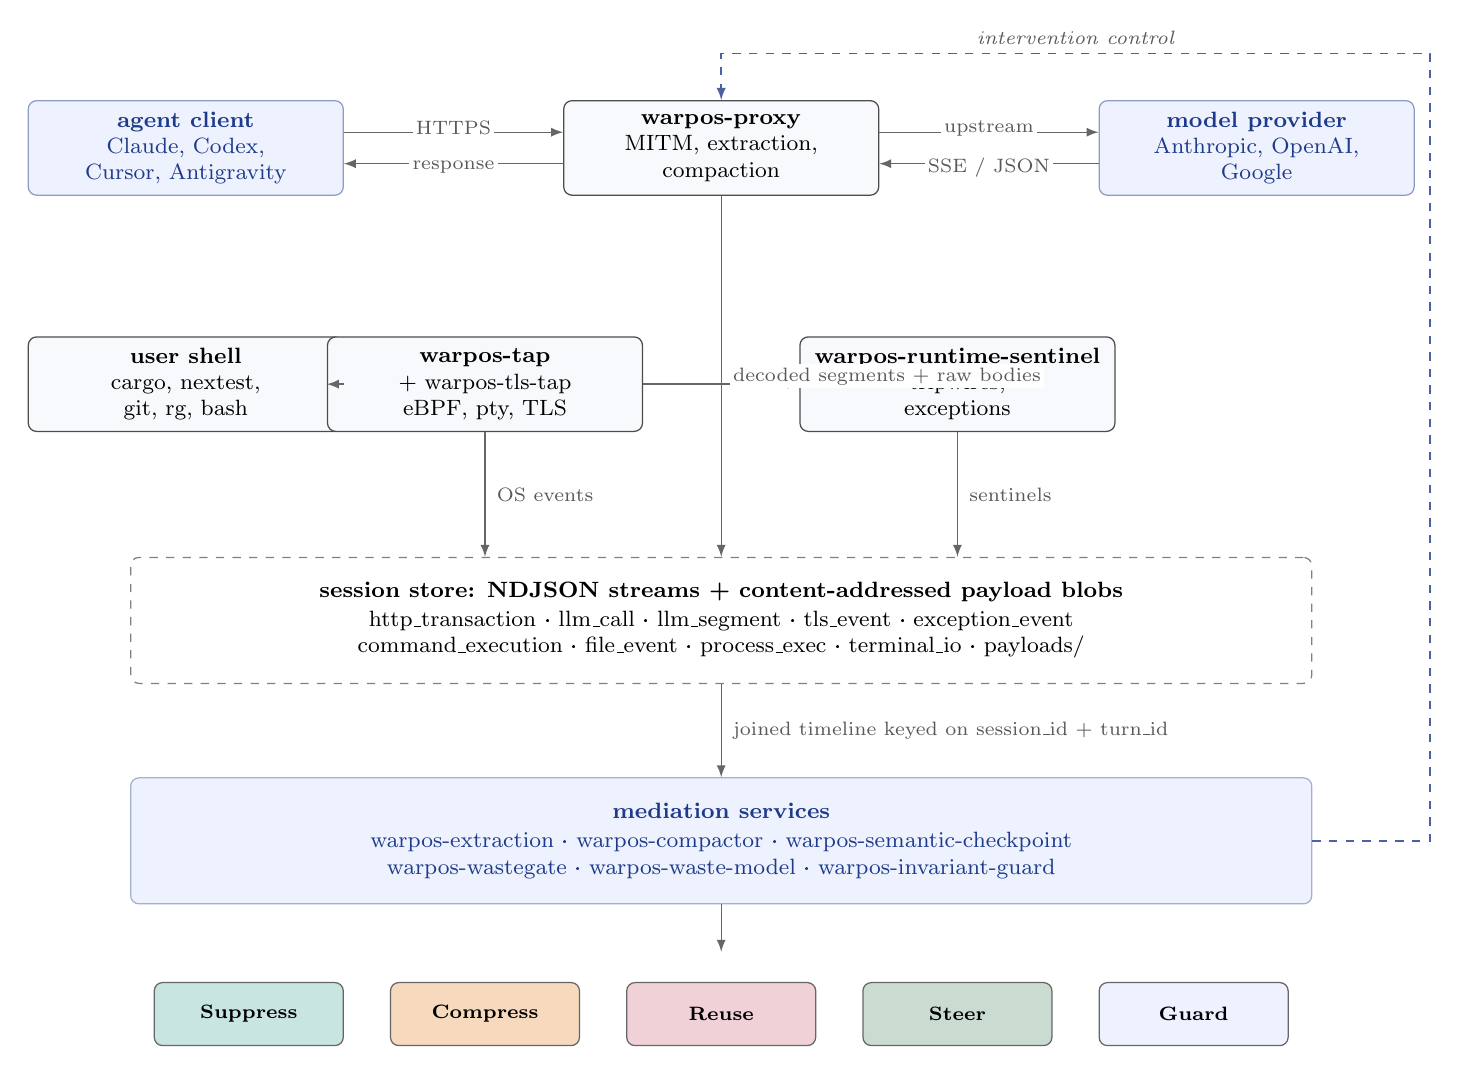
\begin{tikzpicture}[
    x=1mm, y=1mm,
    every node/.style  = {font=\footnotesize, align=center, inner sep=0pt},
    box/.style         = {draw=black!60, line width=0.45pt, rounded corners=3pt,
                          inner sep=3pt, fill=white},
    actor/.style       = {box, fill=accentSoft, draw=accent!50, text=accent,
                          minimum width=40mm, minimum height=12mm},
    service/.style     = {box, fill=tableStripe, draw=black!70,
                          minimum width=40mm, minimum height=12mm},
    store/.style       = {box, fill=white, draw=black!50, dashed,
                          minimum width=150mm, minimum height=16mm},
    services/.style    = {box, fill=tableHeaderBg, draw=accent!40, text=accent,
                          minimum width=150mm, minimum height=16mm},
    stage/.style       = {box, minimum width=24mm, minimum height=8mm,
                          font=\scriptsize\bfseries},
    arrow/.style       = {-latex, draw=black!60, line width=0.5pt},
    ctlarrow/.style    = {-latex, draw=accent!80, line width=0.55pt, dashed},
    lbl/.style         = {font=\scriptsize, fill=white, text=black!65,
                          inner sep=1.2pt},
  ]

  %% Row 1: network layer (y = 130)
  \node[actor]   (agent)    at ( 22,130) {\textbf{agent client}\\Claude, Codex,\\Cursor, Antigravity};
  \node[service] (proxy)    at ( 90,130) {\textbf{warpos-proxy}\\MITM, extraction,\\compaction};
  \node[actor]   (provider) at (158,130) {\textbf{model provider}\\Anthropic, OpenAI,\\Google};

  %% Row 2: OS layer (y = 100)
  %% Deliberate asymmetry: tap is shifted LEFT of proxy and sentinel is
  %% shifted RIGHT so the proxy -> store arrow can drop straight down the
  %% centerline without crossing any row-2 node.
  \node[service] (shell)    at ( 22,100) {\textbf{user shell}\\cargo, nextest,\\git, rg, bash};
  \node[service] (tap)      at ( 60,100) {\textbf{warpos-tap}\\+ warpos-tls-tap\\eBPF, pty, TLS};
  \node[service] (sentinel) at (120,100) {\textbf{warpos-runtime-sentinel}\\tripwires,\\exceptions};

  %% Row 3: session store (y = 70)
  \node[store] (store) at (90,70)
    {\textbf{session store: NDJSON streams + content-addressed payload blobs}\\[1pt]
     \footnotesize http\_transaction \textperiodcentered{} llm\_call \textperiodcentered{} llm\_segment \textperiodcentered{} tls\_event \textperiodcentered{} exception\_event\\
     \footnotesize command\_execution \textperiodcentered{} file\_event \textperiodcentered{} process\_exec \textperiodcentered{} terminal\_io \textperiodcentered{} payloads/};

  %% Row 4: mediation services (y = 42)
  \node[services] (services) at (90,42)
    {\textbf{mediation services}\\[1pt]
     \footnotesize warpos-extraction \textperiodcentered{} warpos-compactor \textperiodcentered{} warpos-semantic-checkpoint\\
     \footnotesize warpos-wastegate \textperiodcentered{} warpos-waste-model \textperiodcentered{} warpos-invariant-guard};

  %% Row 5: five cascade stages (y = 20)
  \node[stage, fill=envBar2!30]  (s1) at ( 30,20) {Suppress};
  \node[stage, fill=envBar1!35]  (s2) at ( 60,20) {Compress};
  \node[stage, fill=envBar0!25]  (s3) at ( 90,20) {Reuse};
  \node[stage, fill=envBar3!25]  (s4) at (120,20) {Steer};
  \node[stage, fill=accentSoft]  (s5) at (150,20) {Guard};

  %% Row 1 horizontal arrows (two-way, offset vertically so labels stack)
  \draw[arrow] ([yshift= 2mm]agent.east)    -- ([yshift= 2mm]proxy.west);
  \draw[arrow] ([yshift=-2mm]proxy.west)    -- ([yshift=-2mm]agent.east);
  \node[lbl] at (56,132.5) {HTTPS};
  \node[lbl] at (56,127.5) {response};

  \draw[arrow] ([yshift= 2mm]proxy.east)    -- ([yshift= 2mm]provider.west);
  \draw[arrow] ([yshift=-2mm]provider.west) -- ([yshift=-2mm]proxy.east);
  \node[lbl] at (124,132.5) {upstream};
  \node[lbl] at (124,127.5) {SSE / JSON};

  %% Row 2 horizontal arrows
  \draw[arrow] (shell.east) -- (tap.west);
  \draw[arrow] (tap.east)   -- (sentinel.west);

  %% Three parallel vertical arrows into the session store.
  \draw[arrow] (proxy.south)    -- node[lbl, right=1mm]{decoded segments + raw bodies}
                                   (store.north -| proxy.south);
  \draw[arrow] (tap.south)      -- node[lbl, right=1mm]{OS events}
                                   (store.north -| tap.south);
  \draw[arrow] (sentinel.south) -- node[lbl, right=1mm]{sentinels}
                                   (store.north -| sentinel.south);

  %% Store -> mediation services
  \draw[arrow] (store.south) -- node[lbl, right=1mm]{joined timeline keyed on session\_id + turn\_id}
                                (services.north);

  %% Services -> cascade row (a single short drop; cascade boxes float below)
  \draw[arrow] (services.south) -- ($(services.south)+(0,-6)$);

  %% Intervention-control loop. Routed outside the main flow:
  %% services.east -> right margin -> up over the top -> down into proxy.north
  \draw[ctlarrow] (services.east) -- (180,42) -- (180,142) -- (90,142) -- (proxy.north);
  \node[lbl] at (135,144) {\itshape intervention control};

\end{tikzpicture}
 from main.tex inside a figure*
%% environment. A standalone compile wrapper lives in
%% warpos-diagram-standalone.tex (same diagram, with a minimal preamble so it
%% can be built on its own and handed to an outside editor).
%%
%% Relies on the following TikZ libraries already loaded in main.tex:
%%   \usetikzlibrary{positioning,patterns}
%% and on the colors accent, accentSoft, tableStripe, tableHeaderBg, and the
%% envBar0/1/2/3 ramp used elsewhere in the paper.
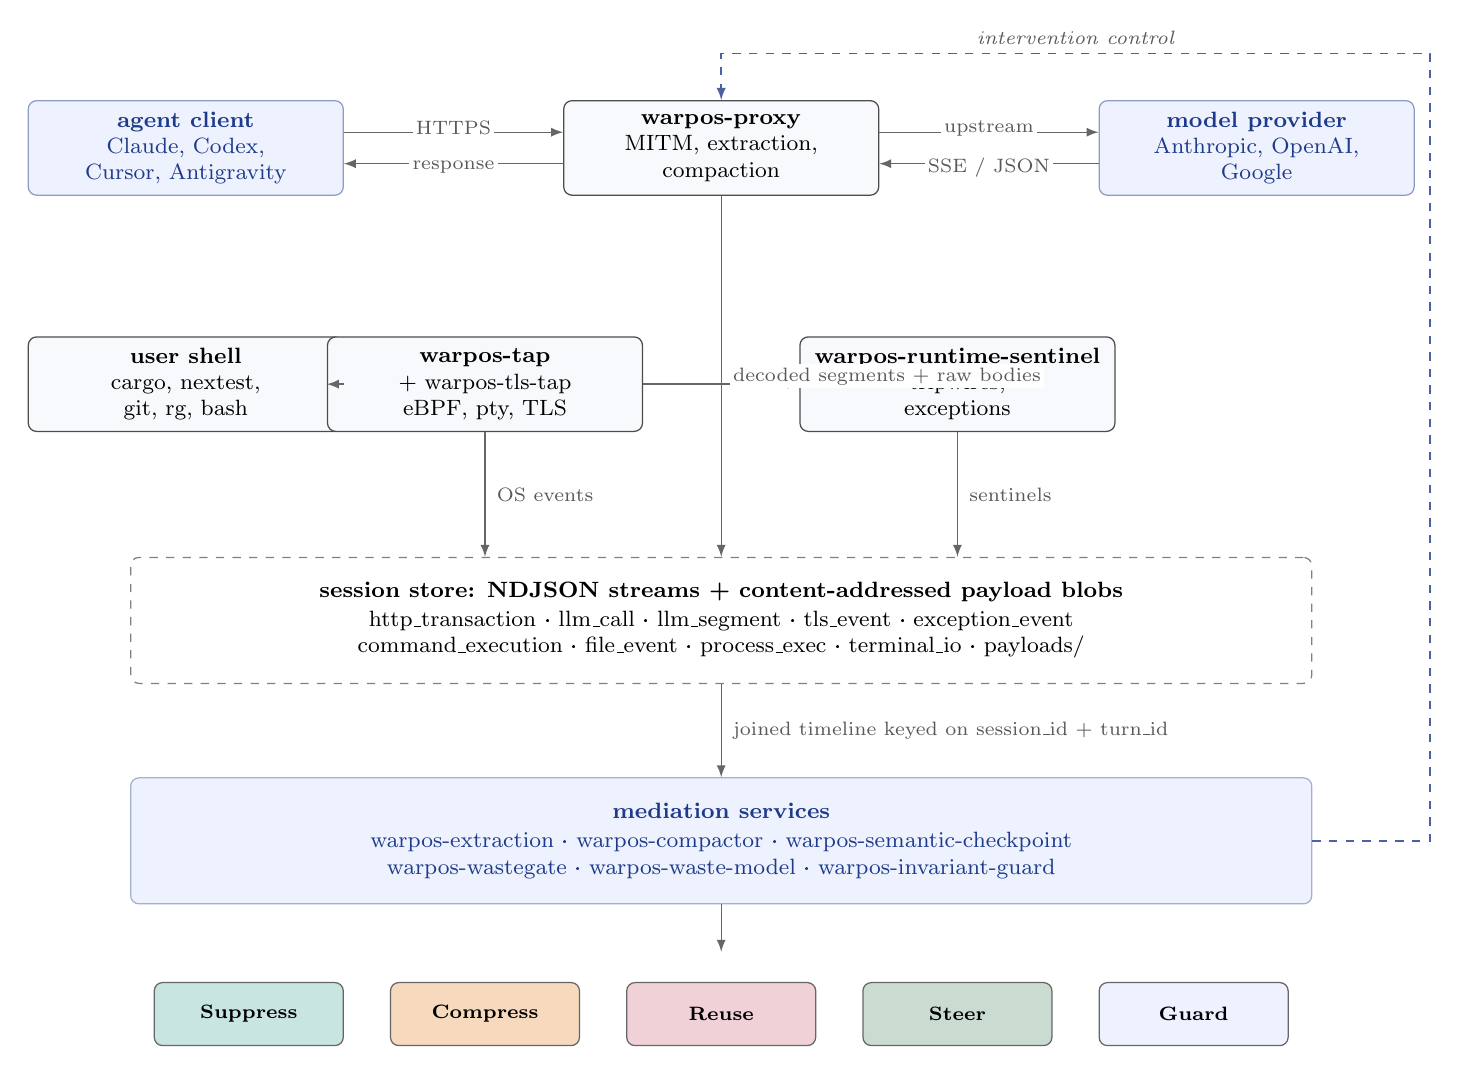
\begin{tikzpicture}[
    x=1mm, y=1mm,
    every node/.style  = {font=\footnotesize, align=center, inner sep=0pt},
    box/.style         = {draw=black!60, line width=0.45pt, rounded corners=3pt,
                          inner sep=3pt, fill=white},
    actor/.style       = {box, fill=accentSoft, draw=accent!50, text=accent,
                          minimum width=40mm, minimum height=12mm},
    service/.style     = {box, fill=tableStripe, draw=black!70,
                          minimum width=40mm, minimum height=12mm},
    store/.style       = {box, fill=white, draw=black!50, dashed,
                          minimum width=150mm, minimum height=16mm},
    services/.style    = {box, fill=tableHeaderBg, draw=accent!40, text=accent,
                          minimum width=150mm, minimum height=16mm},
    stage/.style       = {box, minimum width=24mm, minimum height=8mm,
                          font=\scriptsize\bfseries},
    arrow/.style       = {-latex, draw=black!60, line width=0.5pt},
    ctlarrow/.style    = {-latex, draw=accent!80, line width=0.55pt, dashed},
    lbl/.style         = {font=\scriptsize, fill=white, text=black!65,
                          inner sep=1.2pt},
  ]

  %% Row 1: network layer (y = 130)
  \node[actor]   (agent)    at ( 22,130) {\textbf{agent client}\\Claude, Codex,\\Cursor, Antigravity};
  \node[service] (proxy)    at ( 90,130) {\textbf{warpos-proxy}\\MITM, extraction,\\compaction};
  \node[actor]   (provider) at (158,130) {\textbf{model provider}\\Anthropic, OpenAI,\\Google};

  %% Row 2: OS layer (y = 100)
  %% Deliberate asymmetry: tap is shifted LEFT of proxy and sentinel is
  %% shifted RIGHT so the proxy -> store arrow can drop straight down the
  %% centerline without crossing any row-2 node.
  \node[service] (shell)    at ( 22,100) {\textbf{user shell}\\cargo, nextest,\\git, rg, bash};
  \node[service] (tap)      at ( 60,100) {\textbf{warpos-tap}\\+ warpos-tls-tap\\eBPF, pty, TLS};
  \node[service] (sentinel) at (120,100) {\textbf{warpos-runtime-sentinel}\\tripwires,\\exceptions};

  %% Row 3: session store (y = 70)
  \node[store] (store) at (90,70)
    {\textbf{session store: NDJSON streams + content-addressed payload blobs}\\[1pt]
     \footnotesize http\_transaction \textperiodcentered{} llm\_call \textperiodcentered{} llm\_segment \textperiodcentered{} tls\_event \textperiodcentered{} exception\_event\\
     \footnotesize command\_execution \textperiodcentered{} file\_event \textperiodcentered{} process\_exec \textperiodcentered{} terminal\_io \textperiodcentered{} payloads/};

  %% Row 4: mediation services (y = 42)
  \node[services] (services) at (90,42)
    {\textbf{mediation services}\\[1pt]
     \footnotesize warpos-extraction \textperiodcentered{} warpos-compactor \textperiodcentered{} warpos-semantic-checkpoint\\
     \footnotesize warpos-wastegate \textperiodcentered{} warpos-waste-model \textperiodcentered{} warpos-invariant-guard};

  %% Row 5: five cascade stages (y = 20)
  \node[stage, fill=envBar2!30]  (s1) at ( 30,20) {Suppress};
  \node[stage, fill=envBar1!35]  (s2) at ( 60,20) {Compress};
  \node[stage, fill=envBar0!25]  (s3) at ( 90,20) {Reuse};
  \node[stage, fill=envBar3!25]  (s4) at (120,20) {Steer};
  \node[stage, fill=accentSoft]  (s5) at (150,20) {Guard};

  %% Row 1 horizontal arrows (two-way, offset vertically so labels stack)
  \draw[arrow] ([yshift= 2mm]agent.east)    -- ([yshift= 2mm]proxy.west);
  \draw[arrow] ([yshift=-2mm]proxy.west)    -- ([yshift=-2mm]agent.east);
  \node[lbl] at (56,132.5) {HTTPS};
  \node[lbl] at (56,127.5) {response};

  \draw[arrow] ([yshift= 2mm]proxy.east)    -- ([yshift= 2mm]provider.west);
  \draw[arrow] ([yshift=-2mm]provider.west) -- ([yshift=-2mm]proxy.east);
  \node[lbl] at (124,132.5) {upstream};
  \node[lbl] at (124,127.5) {SSE / JSON};

  %% Row 2 horizontal arrows
  \draw[arrow] (shell.east) -- (tap.west);
  \draw[arrow] (tap.east)   -- (sentinel.west);

  %% Three parallel vertical arrows into the session store.
  \draw[arrow] (proxy.south)    -- node[lbl, right=1mm]{decoded segments + raw bodies}
                                   (store.north -| proxy.south);
  \draw[arrow] (tap.south)      -- node[lbl, right=1mm]{OS events}
                                   (store.north -| tap.south);
  \draw[arrow] (sentinel.south) -- node[lbl, right=1mm]{sentinels}
                                   (store.north -| sentinel.south);

  %% Store -> mediation services
  \draw[arrow] (store.south) -- node[lbl, right=1mm]{joined timeline keyed on session\_id + turn\_id}
                                (services.north);

  %% Services -> cascade row (a single short drop; cascade boxes float below)
  \draw[arrow] (services.south) -- ($(services.south)+(0,-6)$);

  %% Intervention-control loop. Routed outside the main flow:
  %% services.east -> right margin -> up over the top -> down into proxy.north
  \draw[ctlarrow] (services.east) -- (180,42) -- (180,142) -- (90,142) -- (proxy.north);
  \node[lbl] at (135,144) {\itshape intervention control};

\end{tikzpicture}
 from main.tex inside a figure*
%% environment. A standalone compile wrapper lives in
%% warpos-diagram-standalone.tex (same diagram, with a minimal preamble so it
%% can be built on its own and handed to an outside editor).
%%
%% Relies on the following TikZ libraries already loaded in main.tex:
%%   \usetikzlibrary{positioning,patterns}
%% and on the colors accent, accentSoft, tableStripe, tableHeaderBg, and the
%% envBar0/1/2/3 ramp used elsewhere in the paper.
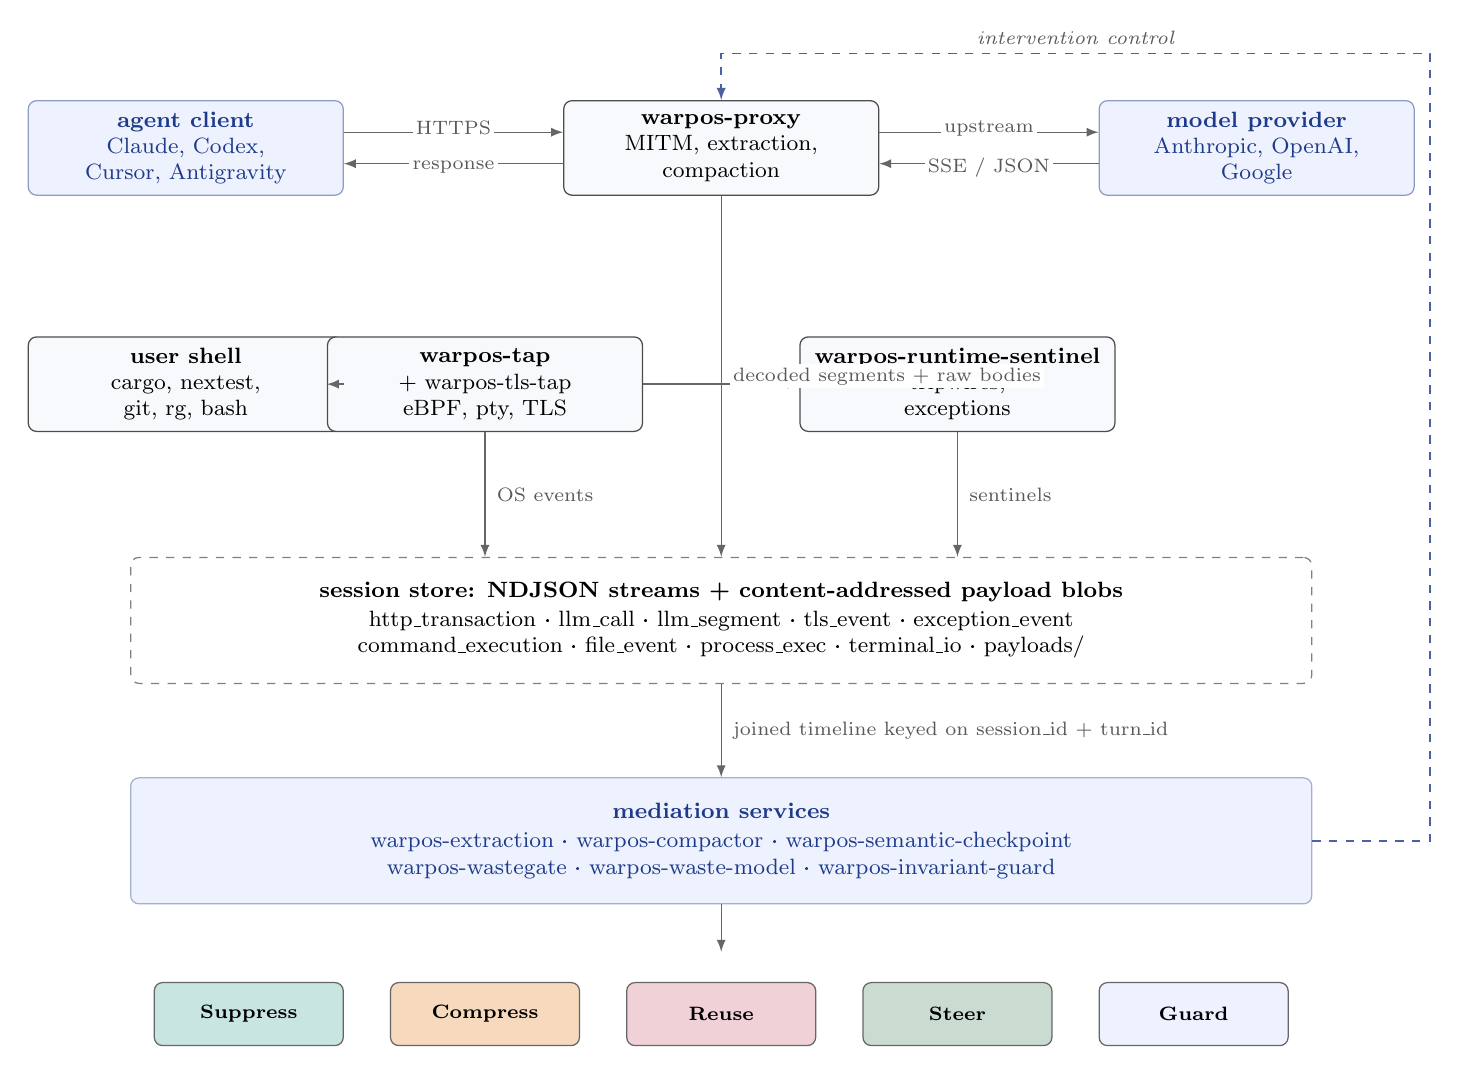
\begin{tikzpicture}[
    x=1mm, y=1mm,
    every node/.style  = {font=\footnotesize, align=center, inner sep=0pt},
    box/.style         = {draw=black!60, line width=0.45pt, rounded corners=3pt,
                          inner sep=3pt, fill=white},
    actor/.style       = {box, fill=accentSoft, draw=accent!50, text=accent,
                          minimum width=40mm, minimum height=12mm},
    service/.style     = {box, fill=tableStripe, draw=black!70,
                          minimum width=40mm, minimum height=12mm},
    store/.style       = {box, fill=white, draw=black!50, dashed,
                          minimum width=150mm, minimum height=16mm},
    services/.style    = {box, fill=tableHeaderBg, draw=accent!40, text=accent,
                          minimum width=150mm, minimum height=16mm},
    stage/.style       = {box, minimum width=24mm, minimum height=8mm,
                          font=\scriptsize\bfseries},
    arrow/.style       = {-latex, draw=black!60, line width=0.5pt},
    ctlarrow/.style    = {-latex, draw=accent!80, line width=0.55pt, dashed},
    lbl/.style         = {font=\scriptsize, fill=white, text=black!65,
                          inner sep=1.2pt},
  ]

  %% Row 1: network layer (y = 130)
  \node[actor]   (agent)    at ( 22,130) {\textbf{agent client}\\Claude, Codex,\\Cursor, Antigravity};
  \node[service] (proxy)    at ( 90,130) {\textbf{warpos-proxy}\\MITM, extraction,\\compaction};
  \node[actor]   (provider) at (158,130) {\textbf{model provider}\\Anthropic, OpenAI,\\Google};

  %% Row 2: OS layer (y = 100)
  %% Deliberate asymmetry: tap is shifted LEFT of proxy and sentinel is
  %% shifted RIGHT so the proxy -> store arrow can drop straight down the
  %% centerline without crossing any row-2 node.
  \node[service] (shell)    at ( 22,100) {\textbf{user shell}\\cargo, nextest,\\git, rg, bash};
  \node[service] (tap)      at ( 60,100) {\textbf{warpos-tap}\\+ warpos-tls-tap\\eBPF, pty, TLS};
  \node[service] (sentinel) at (120,100) {\textbf{warpos-runtime-sentinel}\\tripwires,\\exceptions};

  %% Row 3: session store (y = 70)
  \node[store] (store) at (90,70)
    {\textbf{session store: NDJSON streams + content-addressed payload blobs}\\[1pt]
     \footnotesize http\_transaction \textperiodcentered{} llm\_call \textperiodcentered{} llm\_segment \textperiodcentered{} tls\_event \textperiodcentered{} exception\_event\\
     \footnotesize command\_execution \textperiodcentered{} file\_event \textperiodcentered{} process\_exec \textperiodcentered{} terminal\_io \textperiodcentered{} payloads/};

  %% Row 4: mediation services (y = 42)
  \node[services] (services) at (90,42)
    {\textbf{mediation services}\\[1pt]
     \footnotesize warpos-extraction \textperiodcentered{} warpos-compactor \textperiodcentered{} warpos-semantic-checkpoint\\
     \footnotesize warpos-wastegate \textperiodcentered{} warpos-waste-model \textperiodcentered{} warpos-invariant-guard};

  %% Row 5: five cascade stages (y = 20)
  \node[stage, fill=envBar2!30]  (s1) at ( 30,20) {Suppress};
  \node[stage, fill=envBar1!35]  (s2) at ( 60,20) {Compress};
  \node[stage, fill=envBar0!25]  (s3) at ( 90,20) {Reuse};
  \node[stage, fill=envBar3!25]  (s4) at (120,20) {Steer};
  \node[stage, fill=accentSoft]  (s5) at (150,20) {Guard};

  %% Row 1 horizontal arrows (two-way, offset vertically so labels stack)
  \draw[arrow] ([yshift= 2mm]agent.east)    -- ([yshift= 2mm]proxy.west);
  \draw[arrow] ([yshift=-2mm]proxy.west)    -- ([yshift=-2mm]agent.east);
  \node[lbl] at (56,132.5) {HTTPS};
  \node[lbl] at (56,127.5) {response};

  \draw[arrow] ([yshift= 2mm]proxy.east)    -- ([yshift= 2mm]provider.west);
  \draw[arrow] ([yshift=-2mm]provider.west) -- ([yshift=-2mm]proxy.east);
  \node[lbl] at (124,132.5) {upstream};
  \node[lbl] at (124,127.5) {SSE / JSON};

  %% Row 2 horizontal arrows
  \draw[arrow] (shell.east) -- (tap.west);
  \draw[arrow] (tap.east)   -- (sentinel.west);

  %% Three parallel vertical arrows into the session store.
  \draw[arrow] (proxy.south)    -- node[lbl, right=1mm]{decoded segments + raw bodies}
                                   (store.north -| proxy.south);
  \draw[arrow] (tap.south)      -- node[lbl, right=1mm]{OS events}
                                   (store.north -| tap.south);
  \draw[arrow] (sentinel.south) -- node[lbl, right=1mm]{sentinels}
                                   (store.north -| sentinel.south);

  %% Store -> mediation services
  \draw[arrow] (store.south) -- node[lbl, right=1mm]{joined timeline keyed on session\_id + turn\_id}
                                (services.north);

  %% Services -> cascade row (a single short drop; cascade boxes float below)
  \draw[arrow] (services.south) -- ($(services.south)+(0,-6)$);

  %% Intervention-control loop. Routed outside the main flow:
  %% services.east -> right margin -> up over the top -> down into proxy.north
  \draw[ctlarrow] (services.east) -- (180,42) -- (180,142) -- (90,142) -- (proxy.north);
  \node[lbl] at (135,144) {\itshape intervention control};

\end{tikzpicture}

\caption{WarpOS network topology and dataflow. The agent client talks to the model provider through \texttt{warpos-proxy}, which terminates TLS using a local root certificate, normalizes gzip/brotli/zstd and SSE framing, and writes both decoded segments and content-addressed raw bodies to a session store. An OS-level tap (eBPF-assisted \texttt{warpos-tap} plus \texttt{warpos-tls-tap}) and a runtime sentinel write process, file, command, and tripwire events to the same store, keyed by \texttt{session\_id} and \texttt{turn\_id}. Mediation services read the joined timeline and drive the five cascade stages (Suppress, Compress, Reuse, Steer, Guard), which loop intervention control back into the proxy. Dashed arrows carry intervention decisions; solid arrows carry traffic or telemetry.}
\label{fig:warpos-arch}
\end{figure*}

\subsection{Data Families}
\label{app:warpos-data}

The session store contains one directory per session with parallel NDJSON streams and a content-addressed payload blob store. \texttt{http\_transaction.ndjson} captures every normalized request/response pair with decoded body and scrub-rule projection; \texttt{llm\_call.ndjson} records per-turn model, tokens, scope, call class, prompt fingerprint, and tool-schema hash; \texttt{llm\_segment.ndjson} splits each turn into typed segments (\texttt{system\_message}, \texttt{user\_message}, \texttt{tool\_schema}, \texttt{tool\_call}, \texttt{tool\_result}, \texttt{visible\_reasoning}, \texttt{runtime\_error\_text}); \texttt{tls\_event.ndjson} records TLS handshake observations for traffic outside MITM scope; \texttt{exception\_event.ndjson} carries runtime-sentinel tripwires. On the OS side, \texttt{command\_execution.ndjson} carries argv, cwd, exit code, and stdout/stderr references paired with the model turn that initiated them; \texttt{file\_event.ndjson} carries path, op, bytes, and content hash; \texttt{process\_exec.ndjson} and \texttt{terminal\_io.ndjson} complete the process/pty view. The \texttt{payloads/} subdirectory keys raw request and response bodies by SHA-256 so every rewrite has a falsifiable recovery path.

\subsection{MITM Addon Pipeline}
\label{app:warpos-mitm}

The reference \texttt{mitmproxy} addon attaches at four hook points: \texttt{request} (pre-dial), \texttt{response} (post-dial, pre-body), body-parse (for both request and response segments), and session-finalize. At each stage the addon reads one or more per-agent extraction rules and writes one or more NDJSON records plus, if applicable, a content-addressed payload blob. Segmentation is the most consequential step: a single LLM response turn is decomposed into a typed sequence of segments, each carrying a \texttt{source} field recording where in the provider envelope it came from. Segmentation is what lets the Compress stage emit a typed packet in place of a \texttt{tool\_result} without mutating the enclosing turn envelope, and what lets the Guard stage ask whether a claim of ``tests passed'' is supported by a \texttt{command\_execution} row with \texttt{exit\_code==0} in the same turn. Normalization handles content encoding (gzip, brotli, zstd), server-sent-events framing, and provider-specific envelope quirks; payloads are decoded before hashing so two semantically identical responses with different compression produce the same \texttt{payload\_hash}.

\subsection{Extraction Rules and Provider Normalization}
\label{app:warpos-extraction}

Per-agent \texttt{extraction\_rules.json} files (schema version 2) are the dispatch table that makes the rest of the stack provider-neutral. Each file has seven rule groups: \emph{provider rules} (host/path/user-agent to provider family), \emph{scope rules} (path to scope), \emph{call-class rules} (call class per path), \emph{usage rules} (where to read token counts), \emph{model and feature rules} (normalizing identity), \emph{payload projection rules} (what sub-objects to lift into \texttt{llm\_segment}), and \emph{scrub rules} (request-scoped fields to strip before fingerprinting). These rules are why the same five cascade stages present uniformly across Claude (Anthropic Messages), Codex (ChatGPT backend), Cursor (\texttt{aiserver.v1} gRPC-web), and Antigravity (Gemini \texttt{/v1internal}).

\subsection{Hazard Model and Intervention Dispatch}
\label{app:warpos-hazard}

The learned part of the stack materializes state/action rows with $\sim$219 features; the feature manifest marks each feature as \texttt{runtime\_safe}, \texttt{hindsight\_only}, or \texttt{oracle\_only}, and only runtime-safe features may be consumed online. The training script fits five gradient-boosted hazard heads plus one utility head. The five PRIMARY labels are: next-step illegal touch; next-three-steps requires widen lease; current state should switch to patch-proposal mode; current run needs hard-freeze of boundary writes; and next-five-steps validation blowup. The canonical action space is seven tokens:
\begin{itemize}\itemsep 1pt \parsep 1pt \topsep 2pt
  \item \texttt{continue} (no intervention)
  \item \texttt{trap\_now}
  \item \texttt{force\_lease\_now}
  \item \texttt{hard\_freeze\_\allowbreak boundary\_writes}
  \item \texttt{switch\_to\_\allowbreak patch\_proposal\_now}
  \item \texttt{suppress\_\allowbreak broad\_\allowbreak validation\_now}
  \item \texttt{reveal\_next\_\allowbreak probe\_now}
\end{itemize}
At runtime, the hazard service extracts the runtime-safe feature subset from the live session, scores the five heads, computes adjusted utility per action, and dispatches only when the top non-\texttt{continue} action exceeds \texttt{continue} plus an \texttt{abstain\_margin} (default 50). Below that margin, the row is logged but no action fires; this is the shadow-mode discipline the paper cites repeatedly. The current offline replay result is 18 of 34 invalid runs prevented on ISSUE-05, with 1\,242\,298 optimistic tokens saved. That number is the ceiling that scales by \texttt{abstain\_margin} for online projections throughout~\S\ref{sec:runtime}; it is not a deployment outcome, and generalization to other issue families requires rebuilding the dataset from those runsets.

\subsection{Storage, Retention, and Replay}
\label{app:warpos-storage}

Session directories are append-only: NDJSON streams never mutate in place, and payload blobs are write-once and deduplicated by content hash. A session manifest is written at teardown recording session identity, policy hashes, and stream counts; replaying a past session under a different policy produces a different manifest hash and can never be silently confused with the original. Retention is operator-controlled and defaults to session-scope. Cross-session deduplication is intrinsically content-addressed and therefore privacy-bounded to what the hash already reveals.

\subsection{Safety, Privacy, and Limitations}
\label{app:warpos-limits}

WarpOS captures traffic and OS events that can contain credentials, tokens, customer data, and source code. Scrub rules strip obvious secrets at extraction time, but the content-addressed payload store holds raw bodies by design and must be managed with the same care as any other credential-adjacent artifact. The mediation plane runs with the user's local permissions; setups that share a workstation across users should run the plane per-user rather than as a system service, and a hardened deployment should run it inside a network namespace with an explicit egress policy.

Three limitations bound every runtime claim in this paper. First, \emph{single-session corpus}: Figure~\ref{fig:warpos-opportunity} uses one session per agent, so session-to-session variance is not yet measured. Second, \emph{single issue family}: hazard-gated steering is grounded in ISSUE-05 offline replay only; generalization to ISSUE-01, ISSUE-03, and ISSUE-04 has not been rerun publicly, and ISSUE-06 through ISSUE-10 remain blueprint. Third, \emph{label coverage debt}: several Guard and Steer interventions still require shadow-mode labels before they can ship. Claims labeled ``projected'' are bounded by these three gaps and should not be read past them.

\bibliographystyle{IEEEtran}
\bibliography{references}

\end{document}
